\documentclass{article}

\usepackage[top=3cm, bottom=3cm, left=3cm,right=3cm]{geometry}
\usepackage[colorinlistoftodos]{todonotes}
\usepackage{graphicx}
\usepackage{amssymb}
\usepackage{amsmath}
\usepackage{bbm}
\usepackage{todonotes}
\usepackage{pdflscape}
\usepackage{caption}
\usepackage{subcaption}
\usepackage[T1]{fontenc}
\usepackage[utf8]{inputenc}
\usepackage{authblk}
\usepackage{pdfpages}
\usepackage{setspace} 
\usepackage{booktabs}
\usepackage{longtable}
\usepackage{float}
\usepackage{tikz}
\usepackage[colorlinks=true,citecolor=blue, linkcolor=blue]{hyperref}
\usepackage{multirow}
\setlength{\tabcolsep}{5pt}
%%\setlength{\parindent}{0pt}
\usepackage[parfill]{parskip}
\renewcommand{\arraystretch}{1.5}

\usepackage{tikz}
\usetikzlibrary{shapes.geometric, arrows}

\tikzstyle{startstop} = [rectangle, rounded corners, minimum width=3cm, minimum height=1.75cm, text centered, draw=black, text width=3cm, fill=red!30]
\tikzstyle{bigrec} = [rectangle, rounded corners, minimum width=8.25cm, minimum height=1.75cm, text centered, draw=black, text width=5cm, fill=blue!30]
\tikzstyle{bigrec2} = [rectangle, rounded corners, minimum width=11.2cm, minimum height=1.75cm, text centered, draw=black, text width=3cm, fill=green!30]


\tikzstyle{arrow} = [thick, ->, >=stealth]
\tikzstyle{darrow} = [thick, <->, >=stealth]

\renewcommand\Affilfont{\itshape\footnotesize}
\def\ci{\perp\!\!\!\perp}

\renewcommand\Affilfont{\itshape\footnotesize}
\linespread{1.5}

% \usepackage{lineno}
% \linenumbers

% Article Guidelines: https://www.nature.com/ncomms/submit/article
% Article Guidelines: https://www.nature.com/documents/ncomms-submission-guide.pdf
% The main text (not including abstract, Methods, References and figure legends) 
% is limited to 5,000 words. The maximum title length is 15 words. The abstract — 
% which should be no more than 150 words long and contain no references — should 
% serve both as a general introduction to the topic and as a brief, non-technical 
% summary of the main results and their implications.

% The main text of an Article should begin with a section headed Introduction 
% of referenced text that expands on the background of the work (some overlap 
% with the abstract is acceptable), followed by sections headed Results, 
% Discussion (if appropriate) and Methods (if appropriate). The Results and 
% Methods sections should be divided by topical subheadings; the Discussion 
% should be succinct and may not contain subheadings. Methods are typically 
% less than 3000 words. Figure legends are limited to 350 words each. As a 
% guide, references should not exceed 70. Footnotes are not used.

% Nature Bibliography style
\usepackage[backend=biber,style=nature]{biblatex}
\addbibresource{Refs.bib} 

%% Label figures and tables Figure SX and Table SX
\renewcommand{\thefigure}{S\arabic{figure}}
\renewcommand{\thetable}{S\arabic{table}}

%%%%%%%%%%%%%
%%% Title %%%
%%%%%%%%%%%%%
% Limit: 15 words
\title{Supplementary material: Substantial but spatially heterogeneous progress in male circumcision for HIV prevention in South Africa}

\author{}
\date{}

%%%%%%%%%%%%%%%%%%%%%%%%%%%%%%%%%%%%%%%%%%%%%%%%%%%%%%%%%%%%%%%%%%
%%%%%%%%%%%%%%%%%%%%%%%%%%%%%%%%%%%%%%%%%%%%%%%%%%%%%%%%%%%%%%%%%%
%%%%%%%%%%%%%%%%%%%%%%%%%%%%%%%%%%%%%%%%%%%%%%%%%%%%%%%%%%%%%%%%%%

\begin{document}

%%%%%%%%%%%%%%%%%%%%%%%%%%%%%%%%%%%%%%%%%%%%%%%%%%%%%%%%%%%%%%%%%%
%%%%%%%%%%%%%%%%%%%%%%%%%%%%%%%%%%%%%%%%%%%%%%%%%%%%%%%%%%%%%%%%%%
%%%%%%%%%%%%%%%%%%%%%%%%%%%%%%%%%%%%%%%%%%%%%%%%%%%%%%%%%%%%%%%%%%

\maketitle

\vspace{-1.5cm}

Matthew L. Thomas\textsuperscript{1,2*},
Khangelani Zuma\textsuperscript{3,4},
Dayanund Loykissoonlal\textsuperscript{5},
Bridget Dube\textsuperscript{6},
Peter Vranken\textsuperscript{7},
Sarah E. Porter\textsuperscript{7},
Katharine Kripke\textsuperscript{8},
Thapelo Seatlhodi\textsuperscript{5,9},
Gesine Meyer-Rath\textsuperscript{10,11},
Leigh F. Johnson\textsuperscript{9},
Jeffrey W. Eaton\textsuperscript{2, 12} \\

\vspace{-0.5cm}
  
\textbf{1} Department of Earth and Environmental Sciences, University of Manchester, Manchester, United Kingdom\\
\textbf{2} MRC Centre for Global Infectious Disease Analysis, School of Public Health, Imperial College London, London, United Kingdom\\
\textbf{3} Human and Social Capabilities Research Division, Human Sciences Research Council,  Pretoria, South Africa\\
\textbf{4} School of Public Health, University of the Witwatersrand, Johannesburg, South Africa\\
\textbf{5} National Department of Health, Pretoria, South Africa\\
\textbf{6} Genesis Analytics, Johannesburg, South Africa\\
\textbf{7} Division of Global HIV and Tuberculosis, Centers for Disease Control and Prevention, Pretoria, South Africa\\
\textbf{8} Avenir Health, Washington, District of Columbia, United States of America\\
\textbf{9} Centre for Infectious Disease Epidemiology and Research, University of Cape Town, Cape Town, South Africa \\
\textbf{10} Health Economics and Epidemiology Research Office, Faculty of Health Sciences, University of Witwatersrand, Johannesburg, South Africa\\
\textbf{11} Department of Global Health, Boston University School of Public Health, Boston, Massachusetts, United Staes of America\\
\textbf{12} Center for Communicable Disease Dynamics, Department of Epidemiology, Harvard T.H. Chan School of Public Health, Boston, Massachusetts, United States of America\\

\vspace{-0.5cm}

* matthew.l.thomas@manchester.ac.uk
\newpage



%%%%%%%%%%%%%%%%%%%%%%%%%%%%%%%%%%%%%%%%%%%%%%%%%%%%%%%%%%%%%%%%%%
%%%%%%%%%%%%%%%%%%%%%%%%%%%%%%%%%%%%%%%%%%%%%%%%%%%%%%%%%%%%%%%%%%
%%%%%%%%%%%%%%%%%%%%%%%%%%%%%%%%%%%%%%%%%%%%%%%%%%%%%%%%%%%%%%%%%%

\begin{appendix}

%%%%%%%%%%%%%%%%%%%%%%%%%%%%%%%%%%%%%%%%%%%%%%%%%%%%%%%%%%
%%%% Resetting figure and table count for the appendix %%%
%%%%%%%%%%%%%%%%%%%%%%%%%%%%%%%%%%%%%%%%%%%%%%%%%%%%%%%%%%
%\setcounter{figure}{0} \renewcommand{\thefigure}{A.\arabic{figure}}
%\setcounter{table}{0} \renewcommand{\thetable}{A.\arabic{table}}

\newpage

\tableofcontents

\newpage

%%%%%%%%%%%%%%%%%%%%%%%%%%%%%%%%%%%%%%%%%%%%%%%%%%%%%%%%%%%%%%%%%%
%%%%%%%%%%%%%%%%%%%%%%%%%%%%%%%%%%%%%%%%%%%%%%%%%%%%%%%%%%%%%%%%%%
%%%%%%%%%%%%%%%%%%%%%%%%%%%%%%%%%%%%%%%%%%%%%%%%%%%%%%%%%%%%%%%%%%

\section{Statistical Methods}
\label{sec::methods}

%%%%%%%%%%%%%%%%%%%%%%%%%%%%%%%%%%%%%%%%%%%%%%%%%%%%%%%%%%%%%%%%%%
%%%%%%%%%%%%%%%%%%%%%%%%%%%%%%%%%%%%%%%%%%%%%%%%%%%%%%%%%%%%%%%%%%
%%%%%%%%%%%%%%%%%%%%%%%%%%%%%%%%%%%%%%%%%%%%%%%%%%%%%%%%%%%%%%%%%%

\noindent Using a Bayesian hierarchical model with small area estimation methods, we modelled probabilities of circumcision stratified by region, age, and time for two types of circumcision: (1) circumcisions that occurred in traditional male initiation ceremonies or for other religious or cultural reasons (TMIC) and (2) circumcisions for non-traditional reasons and/or HIV prevention that take place in a clinical setting using medical methods (MMC-nT). Reflecting recent efforts to encourage adoption of medical methods in TMICs, TMICs were sub-categorised into: (1) traditional circumcisions conducted using non-medical methods (TMC) and (2) circumcisions conducted as part of TMIC but using medical methods (MMC-T), determined by a district- and year-specific probability that TMIC circumcisions were performed as MMC-Ts.\\

\noindent Probabilities of circumcision were estimated using a competing risk discrete time-to-event model \cite{putter2006tutorial}, with estimates of circumcision coverage by type within each cohort calculated using the cumulative incidence. These were combined with data on male population size to calculate the predicted number of circumcisions conducted per year. Likelihood functions were specified for the two data sources to inform parameter calibration: (1) the probability of individual-level observations of circumcision age, type, and year reported by men in national household surveys in a time-to-event framework, and (2) the reported number of medical male circumcisions conducted in each district for HIV prevention among males 10 years and older using a Poisson count model. \\

\noindent Throughout the methods and applications sections, we refer to the following types of circumcision (Figure \ref{fig::modelstr}):
\begin{itemize}
    \item \textbf{MMC-nT:} Medical male circumcisions conducted outside of traditional male initiation ceremonies, representing the large majority of MMC conducted.
    \item \textbf{TMC:} Traditional male circumcisions, assumed to be conducted outside a medical setting for traditional male initiation purposes.
    \item \textbf{MMC-T:} Medical male circumcisions conducted as part of traditional male initiation ceremonies, typically in place of circumcisions that previously would have been conducted as TMC.
\end{itemize}
Useful aggregates of these circumcision types are referred to as:
\begin{itemize}
    \item \textbf{MMC:} All medical male circumcisions (MMC-nT + MMC-T), assumed to be consistent with circumcisions reported through VMMC programme data reporting.
    \item \textbf{TMIC:} All male circumcisions conducted as part of traditional male initiation practices (TMC + MMC-T).
    \item \textbf{MC:} All male circumcisions of any type (MMC-nT + TMC + MMC-T).
\end{itemize}

\begin{figure}[H]
	\centering
	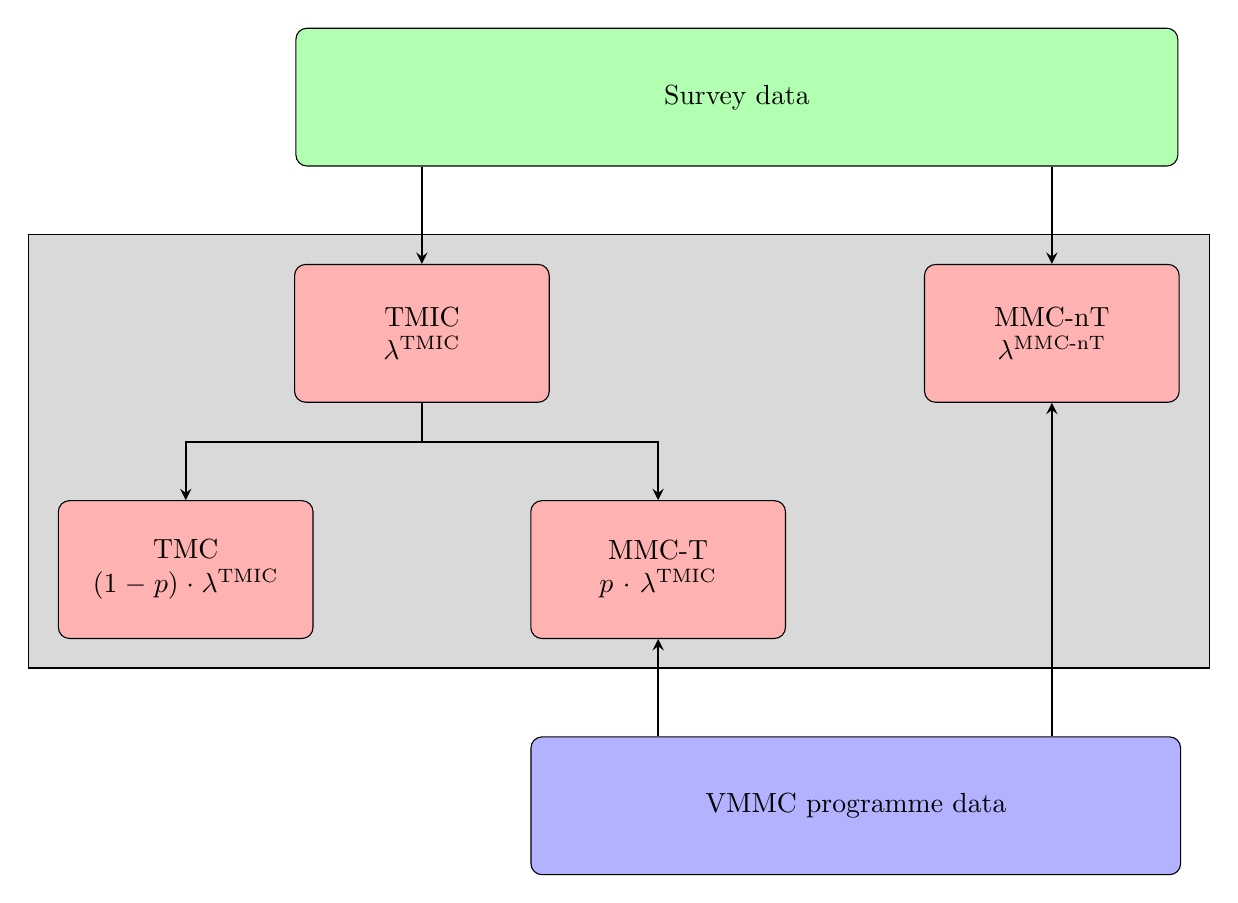
\begin{tikzpicture}[node distance=2cm]
		\draw [black, fill=gray!30] (-9cm,-1.75cm) -- (6cm,-1.75cm) -- (6cm,-7.25cm) -- (-9cm,-7.25cm) -- cycle;
		% Nodes 
		\node (MC) [bigrec2] {Survey data};
		\node (MMC) [startstop, below of = MC, right of = MC, xshift = 2cm, yshift = -1cm] {MMC-nT \\ $\lambda^{\text{MMC-nT}}$};
		\node (TMIC) [startstop, below of = MC, left of = MC, xshift = -2cm, yshift = -1cm] {TMIC \\ $\lambda^{\text{TMIC}}$};
		\node (TMC) [startstop, below of = TMIC, left of = TMIC, xshift = -1cm, yshift = -1cm] {TMC \\ $(1-p)\cdot\lambda^{\text{TMIC}}$};
		\node (MMCT) [startstop, below of = TMIC, right of = TMIC, xshift = 1cm, yshift = -1cm] {MMC-T \\ $p\cdot\lambda^{\text{TMIC}}$};
		\node (ProgData) [bigrec, below of = MC, xshift = 1.51cm, yshift = -7cm] {VMMC programme data};
		% Arrows
		\draw [arrow] (MC.south -| TMIC.north) |- ++(0,-5mm) -| (TMIC.north);
		\draw [arrow] (MC.south -| MMC.north) |- ++(0,-5mm) -| (MMC.north);
		\draw [arrow] (TMIC.south) |- ++(0,-5mm) -| (MMCT.north);
		\draw [arrow] (TMIC.south) |- ++(0,-5mm) -| (TMC.north);
		\draw [arrow] (ProgData.north -| MMC.north) -- (MMC.south);
		\draw [arrow] (ProgData.north -| MMCT.north) -- (MMCT.south);
	\end{tikzpicture}		
	\caption{Schematic representation of types of circumcision included in the model and data sources informing each. TMIC = circumcisions conducted as part of traditional male initiation ceremonies; TMC = traditional male circumcisions (conducted by a non-medical practitioner); MMC-T = medical male circumcision conducted as part of traditional male initiation practices; MMC-nT = medical male circumcision conducted outside the context of traditional male initiation (the majority of VMMC for HIV prevention and other routine medical male circumcision). The parameters $\lambda^{\text{MMC-nT}}$ and $\lambda^{\text{TMIC}}$ represent the probabilities of having an MMC-nT and TMC respectively and $p$ represent the proportion of TMICs conducted as medical methods, as described in Section \ref{sec::competingrisks}.}
	\label{fig::modelstr}
\end{figure}

{\linespread{1} 
\begin{table}[H]
	\small
	\centering	
	\caption{Summary of model inputs and outputs.}
    \label{tab::inputsoutputs}
	\begin{tabular}{| p{0.45\linewidth} | p{0.45\linewidth} |}
		\hline

			\textbf{\underline{Model inputs}} & \textbf{\underline{Model outputs}} \\
			
			{\bf Area hierarchy.} List of administrative areas used for health planning ("districts"), geographic boundaries, and nesting in higher level administrative areas.
			\vspace{5pt}
			
			{\bf Population.} Population estimate stratified by district, sex, and single-year age group (0,1, $\cdots$, 59) covering the period of interest. 
			\vspace{5pt}
			
			{\bf Household surveys.} Data related to age, residence, (self-reported) circumcision status, age at circumcision and type of circumcision (medical/traditional) from recent HIV household surveys. 
			\vspace{5pt}
			
			{\bf VMMC programme data.} Data on number of VMMCs performed for HIV prevention by district and year.
			
		& 
			{\bf Indicators.} The model produces outputs for the following indicators: 
			\begin{itemize}
				\item {\it Probabilities of circumcision}
				\item {\it Circumcision coverage (cumulative incidence)}
				\item {\it Male population}
				\item {\it Number circumcised}
				\item {\it Number uncircumcised}
			\end{itemize}
			\vspace{5pt}
			{\bf Stratifications.} All indicators are stratified according to: 
			\begin{itemize}
				\item {\it Geographic}: 
				\begin{itemize}
					\item All levels of the area hierarchy (e.g. national, province, district)
				\end{itemize}
				\item {\it Age groups}: 
				\begin{itemize}
					\item Single-year age group (0, 1, $\cdots$, 59)
					\item Five-year age groups (0-4, 5-9, $\cdots$, 55-59)
					\item Others (0+, 10+, 15+, 15-24, 10-24, 15-29, 10-29, 15-39, 10-39, 15-49, 10-49 and 25-49)
				\end{itemize}
				\item {\it Type}: 
				\begin{itemize}
					\item MMC-nT
					\item MMC-T
					\item TMC
					\item MMC (MMC-nT + MMC-T)
					\item TMIC (TMC + MMC-T)
					\item Total (MMC + MMC-T + TMC)
				\end{itemize}
				\item {\it Time}: 
				\begin{itemize}
					\item Annual, 2008-2019
				\end{itemize}
			\end{itemize}
			\vspace{5pt}
			{\bf Statistics.} Posterior summary statistics are computed for:
			\begin{itemize}
				\item Point estimates: 
				\begin{itemize}
					\item Mean 
					\item Median
				\end{itemize}
				\item Uncertainty: 
				\begin{itemize}
					\item Standard deviation
					\item 95\% credible interval (quantile-based)
				\end{itemize}
			\end{itemize}\\
		\hline 
	\end{tabular}
\end{table}}

%%%%%%%%%%%%%%%%%%%%%%%%%%%%%%%%%%%%%%%%%%%%%%%%%%%%%%%%%%%%%%%%%%
%%%%%%%%%%%%%%%%%%%%%%%%%%%%%%%%%%%%%%%%%%%%%%%%%%%%%%%%%%%%%%%%%%

\subsection{Process model}
\label{sec::competingrisks}

%%%%%%%%%%%%%%%%%%%%%%%%%%%%%%%%%%%%%%%%%%%%%%%%%%%%%%%%%%%%%%%%%%
%%%%%%%%%%%%%%%%%%%%%%%%%%%%%%%%%%%%%%%%%%%%%%%%%%%%%%%%%%%%%%%%%%

\subsubsection{Probabilities of circumcision per time step}

%%%%%%%%%%%%%%%%%%%%%%%%%%%%%%%%%%%%%%%%%%%%%%%%%%%%%%%%%%%%%%%%%%

Utilising data from household surveys, we modelled the probabilities of becoming circumcised per time step through either TMIC or MMC-nT for individuals residing in region $i \in I = \{1, 2, \ldots, N_I\}$ having an MMC, MMC-nT, MMC-T, TMC, TMIC or MMC at age $a \in A = \{0, 1, 2, \ldots, N_A\}$ and time $t \in T = \{1, 2, \ldots, N_T\}$. \\

\noindent We defined $\lambda^{\text{TMIC}}_{iat}$ as the probability that an individual in region $i$ received TMIC at age $a$ and time step $t$, given they were uncircumcised by age $a-1$ and time $t-1$, 
\begin{equation} 
		\lambda^{\text{TMIC}}_{iat} = \mathbb{P}(\text{TMIC} \; \text{in} \; (i,a,t) \; | \; \text{Uncircumcised in} \; (i,a-1, t-1)). 
	\label{eqn::tmic}
\end{equation}
This was modelled using piece-wise logit-linear function:
\begin{equation*} 
	\text{logit}(\lambda^{\text{TMIC}}_{iat}) = \hat{\alpha} + \hat{\psi_i} + \hat{\phi}_a + \hat{\gamma}_{ia}
\end{equation*}
where $\hat{\alpha}$ is the intercept, $\hat{\psi_i}$ is a regional random effect, $\hat{\phi}_a$ is an age random effect, and $\hat{\gamma}_{ia}$ is an age-space interaction term to allow different age patterns of TMIC  across regions. We assumed that the probability of TMIC was constant over time (i.e. $\lambda^{\text{TMIC}}_{iat} \equiv \lambda^{\text{TMIC}}_{ia}$) as TMIC practices have been relatively stable over time. \\

\noindent Similarly, we defined $\lambda^{\text{MMC-nT}}_{iat}$ as the probability an individual in region $i$ received MMC-nT at age $a$ and time $t$, $\lambda^{\text{MMC-T}}_{iat}$, given they were uncircumcised by age $a-1$ and time $t-1$,  
\begin{equation}
		\lambda^{\text{MMC-nT}}_{iat} = \mathbb{P}(\text{MMC-nT} \; \text{in} \; (i,a,t) \; | \; \text{Uncircumcised in} \; (i,a-1, t-1)),
	\label{eqn::mmc}
\end{equation}
To ensure the overall probability of circumcision $\lambda^{\text{TMIC}}_{iat} + \lambda^{\text{MMC-nT}}_{iat} \leq 1$ for all $i$, $a$ and $t$ in the discrete-time framework, we applied the probability of TMIC  before MMC-nT in each time step, and therefore initially model the probability an individual in region $i$ received MMC-nT at age $a$ and time $t$, $\lambda^{\text{MMC-T}}_{iat}$, given they were uncircumcised by age $a-1$ and time $t-1$ and did not recieve TMIC at age $a$ and time $t$
\begin{equation*}
		\tilde{\lambda}^{\text{MMC-nT}}_{iat} = \mathbb{P}(\text{MMC-nT} \; \text{in} \; (i,a,t) \; | \; \text{Uncircumcised in} \; (i,a-1, t-1) \text{ and no TMIC in} \; (i,a, t))
\end{equation*}
such that
\begin{equation*}
		\lambda^{\text{MMC-nT}}_{iat} = \tilde{\lambda}^{\text{MMC-nT}}_{iat}\cdot (1-\lambda^{\text{TMIC}}_{iat}).
\end{equation*}
The probability $\tilde{\lambda}^{\text{MMC-nT}}_{iat}$ was separated into two processes: (i) paediatric circumcision (for those aged 0--9) and (ii) adolescent and adult circumcision (for those aged 10 and over). VMMC programmes only provide MMCs for HIV prevention to those aged 10 and over, while infant and paediatric medical circumcision tends to occur through cultural or religious practices unrelated to scale-up of VMMC for HIV prevention. Therefore, we modelled $\tilde{\lambda}^{\text{MMC-nT}}_{iat}$ using a piece-wise logit-linear function:
\begin{equation*}
	\text{logit}(\tilde{\lambda}^{\text{MMC-nT}}_{iat}) =
	\begin{cases}
		\bar{\alpha} + \bar{\psi}_i + \bar{\phi}_a + \bar{\gamma}_{ia} & \text{for } 0 \leq a \leq 9\\
		\alpha + \psi_i + \phi_a + \theta_t + \gamma_{ia} + \delta_{at} + \zeta_{it} & \text{for } a \geq 10
	\end{cases} 
\end{equation*}
where $\bar{\alpha}$ and $\alpha$ are intercepts, $\bar{\psi}_i$ and $\psi_i$ are regional random effects, $\theta_i$ are temporal random effects, $\bar{\phi}_a$ and $\phi_a$ are age random effects, $\bar{\gamma}_{ia}$ and $\gamma_{ia}$ are age-space interaction terms to allow for different age patterns of MMC-nTs between regions, for paediatric circumcision and adolescent and adult circumcision respectively. The $\delta_{at}$ is an age-time interaction term to allow for different age patterns of MMC-nTs over time and $\zeta_{it}$ is an space-time interaction term to allow for different uptake of MMC-nTs over time across regions, in adolescent and adult men. Similarly, we assumed that the probabilities of MMC-nT among those aged 0--9 were constant over time, (i.e. $\lambda^{\text{MMC-nT}}_{iat} \equiv \lambda^{\text{MMC-nT}}_{ia}$ when $0\leq a \leq 9$), as paediatric medical circumcision practices are unrelated to VMMC for HIV prevention and are relatively stable. \\

\noindent For individuals circumcised in TMIC, we defined a probability, $p_{iat}$ that circumcision was conducted as a MMC-T versus TMC, specified for region $i$, age $a$, and time $t$. The probability an individual in region $i$ received MMC-T at age $a$ and time $t$, $\lambda^{\text{MMC-T}}_{iat}$ was thus 
\begin{equation}
	\begin{split}
		\lambda^{\text{MMC-T}}_{iat} &= \mathbb{P}(\text{MMC-T} \; \text{in} \; (i,a,t) \; | \; \text{Uncircumcised in} \; (i,a-1, t-1)) \\
		&=p_{iat}\cdot\lambda^{\text{TMIC}}_{iat}
	\end{split}
	\label{eqn::mmct}
\end{equation}
and  the probability an individual in region $i$ received TMIC was
\begin{equation}
	\begin{split}
		\lambda^{\text{TMC}}_{iat} &= \mathbb{P}(\text{TMC} \; \text{in} \; (i,a,t) \; | \; \text{Uncircumcised in} \; (i,a-1, t-1)) \\
		&=(1-p_{iat})\cdot\lambda^{\text{TMIC}}_{iat}
	\end{split}
	\label{eqn::tmc}
\end{equation}
Prior to VMMC programmes, all circumcisions conducted in TMIC were TMC, in which case $p_{iat}=0$. The proportion of TMICs conducted as MMC-Ts may not be identifiable from the survey data, particularly for years since the most recent survey. Thus $p_{iat}>0$ should only be introduced in regions where there is knowledge that MMC-Ts were implemented in TMIC settings. \\

\noindent Taken together, the probability of circumcision of any type, at age $a$ and time $t$ given they were uncircumcised by age $a-1$ and time $t-1$ was 
\begin{equation}
	\begin{split}
	\lambda^{\text{MC}}_{iat} &= \mathbb{P}(\text{MC} \; \text{in} \; (i,a,t) \; | \; \text{Uncircumcised in} \; (i,a-1,t-1)) \\
	              &= \lambda^{\text{TMC}}_{iat} + \lambda^{\text{MMC-T}}_{iat} + \lambda^{\text{MMC-nT}}_{iat} \\ 
	              &= \lambda^{\text{TMIC}}_{ia} + \lambda^{\text{MMC-nT}}_{iat}. 
	\end{split}
	\label{eqn::tot}
\end{equation}
The probability an individual in region $i$ remained uncircumcised at age $a$ and time $t$, given they were uncircumcised by age $a-1$ and time $t-1$, was
\begin{equation}
	\begin{split}
		\lambda^{\text{UC}}_{iat} &= \mathbb{P}(\text{Uncircumcised in}  \; (i,a,t) \; | \; \text{Uncircumcised in} \; (i,a-1, t-1)),\\
		&= 1 - \lambda^{\text{TMIC}}_{iat} - \lambda^{\text{MMC-nT}}_{iat} \\
		&= (1 - \lambda^{\text{TMIC}}_{iat})(1 - \tilde{\lambda}^{\text{MMC-nT}}_{iat})
	\end{split}
	\label{eqn::uncirc}
\end{equation}

%%%%%%%%%%%%%%%%%%%%%%%%%%%%%%%%%%%%%%%%%%%%%%%%%%%%%%%%%%%%%%%%%%

\subsubsection{Cumulative incidence of circumcision}

%%%%%%%%%%%%%%%%%%%%%%%%%%%%%%%%%%%%%%%%%%%%%%%%%%%%%%%%%%%%%%%%%%

The probability $S_{iat}$ of remaining uncircumcised up to age $a$ and time $t$,  typically referred to as the survivor function, was expressed as
\begin{equation}
	\begin{split}
		S_{iat} &= \mathbb{P}(\text{Uncircumcised in} \; (i,a-1,t-1)) \\
				&= \prod_{(0,(t-a))}^{(a-1,t-1)}\lambda^{\text{UC}}_{iat} \\
				&= \lambda^{\text{UC}}_{i,0,t-a}\cdot \lambda^{\text{UC}}_{i,1,t-a+1}\cdot\ldots \cdot\lambda^{\text{UC}}_{i,a-1,t-1}
	\end{split}
	\label{eqn::survfunc}
\end{equation}
The cumulative incidence function (CIF) defines the marginal probability (or proportion/coverage of) individuals who were circumcised by type $k\in K = \{$ MMC, MMC-nT, MMC-T, TMC, TMIC or MMC$\}$ by age $a$ and time $t$, accounting for the competing risk of other circumcision type. This was calculated as the sum of incidence of circumcision by type $k$ at each age up to $a$:
\begin{equation}
	\begin{split}
		\text{CIF}_{iat}^k &= \mathbb{P}(k \; \text{by} \; (i,a,t)) \\
		&= \sum_{(0,(t-a))}^{(a,t)} I^k_{iat}
	\end{split}
	\label{eqn::cuminc}
\end{equation}
where $I^k_{iat}$ is the incidence of circumcision type $k$ in region $i$, age $a$ and time $t$. For types $k \in \{\textrm{TMIC}, \textrm{TMC}, \textrm{MMC-T}\}$, this was defined by the probability of remaining uncircumcised by any type up to age $a$ at time $t$ times the probability of circumcision by type $k$ in year $t$ at age $a$
\begin{equation}
	\begin{split}
		I_{iat}^k &= \mathbb{P}(k \; \text{in} \; (i,a,t)) \\
		       &= \mathbb{P}(k \; \text{in} \; (i,a,t) | \; \text{Uncircumcised in} \; (i,a-1,t-1))\times \\
		       & \;\;\;\;\;\;\;\;\;\;\;\;\;\;\;\;\;\mathbb{P}(\text{Uncircumcised in} \; (i,a-1,t-1)) \\
	    	   &= \lambda_{iat}^k \cdot S_{iat} 
	\end{split}
	\label{eqn::inc}
\end{equation}
The overall incidence and CIF by any circumcision type can be obtained by summing across all circumcision types. The CIF is also often referred to as the `sub-distribution function', due to the fact that the cumulative probability of a particular event $k$ by time $t$ will remain below one \cite{putter2006tutorial}. 

%%%%%%%%%%%%%%%%%%%%%%%%%%%%%%%%%%%%%%%%%%%%%%%%%%%%%%%%%%%%%%%%%%
%%%%%%%%%%%%%%%%%%%%%%%%%%%%%%%%%%%%%%%%%%%%%%%%%%%%%%%%%%%%%%%%%%

\subsection{Programme data model}

%%%%%%%%%%%%%%%%%%%%%%%%%%%%%%%%%%%%%%%%%%%%%%%%%%%%%%%%%%%%%%%%%%
%%%%%%%%%%%%%%%%%%%%%%%%%%%%%%%%%%%%%%%%%%%%%%%%%%%%%%%%%%%%%%%%%%

Utilising data on the number of VMMCs reported, we further informed the probabilities of becoming circumcised by region, age and time step. VMMCs conducted by public health programmes consisted of the total number of MMCs (both MMC-nT and MMC-T) conducted in region $i$ at time $t$ and age group $G=[a_1,a_2]$, $Y_{iGt}$. We modelled number of MMCs, $Y^{\text{MMC-nT}}_{iat}$, and MMC-Ts, $Y^{\text{MMC-T}}_{iat}$ in region $i$, at age $a$ and time $t$ using a Poisson likelihood with means $\mu^{\text{MMC}}_{iat}$ and $\mu^{\text{MMC-T}}_{iat}$ respectively,
\begin{equation*}
    Y^{k}_{iat} \;|\; \mu^{k}_{iat}\sim \text{Poisson}(\mu^{k}_{iat}) \\
	\label{eqn::VMMCPoisson}
\end{equation*}
where $k$ is MMC-T or MMC-nT. The mean $\mu^{k}_{iat}$ is determined by multiplying the male population size in region $i$, at age $a$ and time $t$, $P_{iat}$, the probability of remaining uncircumcised in region $i$, up to age $a$ and time $t$, $S_{iat}$, and the probability of being having a MMC-T or MMC-nT at age $a$ and time $t$ given they were uncircumcised by age $a-1$ and time $t-1$, $\lambda^{\text{MMC-T}}_{iat}$ or $\lambda^{\text{MMC-T}}_{iat}$
\begin{equation*}
    \mu^k_{iat} = P_{iat}\cdot S_{iat} \cdot \lambda^{k}_{iat}.
\end{equation*}
where $k$ is MMC-T or MMC-nT. 
\noindent It then follows that the total number of MMCs conducted in region $i$ at time $t$ and age group $G=[a_1,a_2]$, $Y_{iGt}$ are modelled using 
\begin{equation*}
	\begin{split}
		Y_{iGt} \;|\; \mu_{iat} &\sim \text{Poisson}(\mu_{iGt}) \\
		\mu_{iGt} &= \sum_{a = a_1}^{a_2} \mu^{\text{MMC-nT}}_{iat} + \mu^{\text{MMC-T}}_{iat}.
	\end{split}
\end{equation*}

%%%%%%%%%%%%%%%%%%%%%%%%%%%%%%%%%%%%%%%%%%%%%%%%%%%%%%%%%%%%%%%%%%
%%%%%%%%%%%%%%%%%%%%%%%%%%%%%%%%%%%%%%%%%%%%%%%%%%%%%%%%%%%%%%%%%%

\subsection{Priors}

%%%%%%%%%%%%%%%%%%%%%%%%%%%%%%%%%%%%%%%%%%%%%%%%%%%%%%%%%%%%%%%%%%
%%%%%%%%%%%%%%%%%%%%%%%%%%%%%%%%%%%%%%%%%%%%%%%%%%%%%%%%%%%%%%%%%%

In space, we assigned the random effects $\hat{\psi}_i$, $\bar{\psi}_i$, $\psi_i$, $\hat{\gamma}_{ia}$, $\gamma_{ia}$ and $\zeta_{it}$, intrinsic conditional autoregressive (ICAR) priors \cite{besag1995conditional}. An ICAR model encodes spatial dependence between neighbours, defined as areas that share a common boundary, and allows information to be borrowed across regions, which may be useful in areas where data is sparse or non-existent. For a generic parameter $\beta_i$, an ICAR model assumes that the expected value of $\beta_i$ is a weighted average its neighbours, 
\begin{equation*}
	\beta_i \;|\; \beta_{j}, j \sim i, \tau_{\beta} \sim \text{N}\left(\frac{1}{n_i} \sum_{j \sim i} \beta_j, \frac{1}{n_i\tau_{\beta}} \right) \;\;\; i = 1, 2, 3,\ldots, N_I
\end{equation*}
where $j \sim i$ refers to the neighbours of region $i$, $n_i$ is the number of neighbours and $\tau_{\beta}$ is the marginal precision. The joint distribution may be equivalently expressed as $\boldsymbol{\beta} \sim N(\boldsymbol{0}, \tau_{\beta}^{-1}Q^{-1}_{I})$ where $Q_{I}$ is the precision matrix encoding the adjacency structure of the neighbourhoods. The precision matrix $Q_{I}$ is rank deficient and consequently the prior is improper \cite{rue2005gaussian}. \\

\noindent In time, we assigned the random effects $\theta_t$, $\delta_{at}$ and $\zeta_{it}$ an autoregressive process of order 1 (AR1) priors,
\begin{align*} 
  \beta_{t} \; | \; \beta_{t-1}, \rho_{\beta}, \tau_{\beta} &\sim N(\rho_{\beta} \cdot \beta_{t-1}, \;\; \tau^{-1}_{\beta}) \;\;\;  t = 2, 3,\ldots, N_T \\
  \beta_{1} \; | \; \rho_{\beta}, \tau_{\beta} &\sim N(0, \tau^{-1}_{\beta})  \;\;\;  t = 1
\end{align*}
where $|\rho_{\beta}| < 1$ is an autocorrelation parameters controlling the correlation of the effect of the current age on the previous age and $\tau_{\beta}$ is the precision. The joint distribution may be equivalently expressed as $\boldsymbol{\beta}\; | \; \rho_{\beta}, \tau_{\beta} \sim N(\boldsymbol{0}, \tau_{\beta}^{-1}Q^{-1}_{T}(\rho_{\beta}))$ where $Q_{T}$ is the precision matrix and encodes the first order dependency in time controlled by the autocorrelation parameter $\rho_{\beta}$.\\

\noindent In age, we modelled the random effects $\hat{\phi}_a$, $\bar{\phi}_a$, $\phi_a$, $\hat{\gamma}_{ia}$, $\bar{\gamma}_{ia}$, $\gamma_{ia}$ and $\delta_{at}$ using penalised B-spline functions. For a generic parameter $\beta_a$, penalised B-splines assumes that $\beta_a$ is a sum of basis functions, 
\begin{align*} 
	\beta_a = \sum_{j = 1}^{N_J} w_{j}b_{aj}
\end{align*} 
where $b_{aj}$ are B-spline basis functions with knots placed every five years (at 0, 5, 10 etc.), $N_J$ is the number of splines used and $w_{j}$ are the spline weight parameters to be estimated. The weights $w_{j}$ are penalised using an AR1 process 
\begin{align*} 
  w_{j} \; | \; w_{j-1}, \rho_{w}, \tau_{w} &\sim N(\rho_{w} \cdot w_{j-1}, \;\; \tau^{-1}_{w}) \;\;\;  j = 2, 3,\ldots, N_J \\
  w_{1} \; | \; \rho_{w}, \tau_{w} &\sim N(0, \tau^{-1}_{w}) 
\end{align*}
where $|\rho_{w}| < 1$ is an autocorrelation parameters controlling the correlation of the effect of the current age on the previous age and $\tau_{w}$ is the precision. The joint distribution is given by $\boldsymbol{w}\; | \; \rho_{w}, \tau_{w} \sim N(\boldsymbol{0}, \tau_{w}^{-1}Q^{-1}_{A}(\rho_{w}))$ where $Q_{A}$ is the precision matrix as defined by the smoothed function. Then defining $\boldsymbol{\beta} = W_{\beta}\cdot \boldsymbol{w}$ where $W_{\beta}$ is a design matrix evaluating the basis functions $f_{aj}$ at each age of interest, the joint distribution of $\boldsymbol{\beta}\; | \;\boldsymbol{w}, \; W_{\beta}, \; \rho_{w}, \tau_{w}$ is given by, $\boldsymbol{\beta}\; | \;\boldsymbol{\omega}, \; W_{\beta}, \; \rho_{w}, \tau_{w} \sim N(\boldsymbol{0}, \tau_{w}^{-1}(W_{\beta}\cdot Q^{-1}_{A}(\rho_{w})\cdot W_{\beta}^T))$.\\

\noindent Moreover, the age-space, age-time, and space-time interaction terms ($\hat{\gamma}_{ia}$, $\bar{\gamma}_{ia}$, $\gamma_{ia}$, $\delta_{at}$ and $\zeta_{it}$) are modelled as Type IV interactions as defined by Knorr-Held and Leonard \cite{knorr2000bayesian},
\begin{align*} 
  \hat{\boldsymbol{\gamma}} \; | \; \rho_{\boldsymbol{\hat{\gamma}}}, \tau_{\boldsymbol{\hat{\gamma}}} &\sim N(\boldsymbol{0}, \;\tau^{-1}_{\hat{\gamma}} Q^{-1}_{\hat{\gamma}}) \\
  \bar{\boldsymbol{\gamma}} \; | \; \rho_{\boldsymbol{\bar{\gamma}}}, \tau_{\boldsymbol{\bar{\gamma}}} &\sim N(\boldsymbol{0}, \;\tau^{-1}_{\bar{\gamma}} Q^{-1}_{\bar{\gamma}}) \\
  \boldsymbol{\gamma} \; | \; \rho_{\gamma}, \tau_{\gamma} &\sim N(\boldsymbol{0}, \;\tau^{-1}_{\gamma} Q^{-1}_{\gamma})\\
  \boldsymbol{\delta} \; | \; \rho_{1\delta}, \rho_{2\delta}, \tau_{\delta} &\sim N(\boldsymbol{0}, \;\tau^{-1}_{\delta} Q^{-1}_{\delta})\\
  \boldsymbol{\zeta} \; | \; \rho_{\zeta}, \tau_{\zeta} &\sim N(\boldsymbol{0}, \;\tau^{-1}_{\zeta} Q^{-1}_{\zeta})
\end{align*}
where the precision matrices constructed using Kronecker products 
\begin{align*} 
	Q_{\hat{\gamma}} &= [W_{\hat{\gamma}}\cdot Q_A(\rho_{\hat{\gamma}}) \cdot W^T_{\hat{\gamma}} ]\otimes Q_I\\
	Q_{\bar{\gamma}} &= [W_{\bar{\gamma}}\cdot Q_A(\rho_{\bar{\gamma}}) \cdot W^T_{\bar{\gamma}} ]\otimes Q_I\\
	Q_{\gamma} &= [W_{\gamma}\cdot Q_A(\rho_{\gamma}) \cdot W^T_{\gamma} ]\otimes Q_I\\
	Q_{\delta} &=[W_{\delta}\cdot Q_A(\rho_{1\delta}) \cdot W^T_{\delta} ] \otimes Q_T(\rho_{2\delta})\\
	Q_{\zeta} &=Q_I \otimes Q_T(\rho_{\zeta})
\end{align*}
Here, $Q_I$, $Q_A$ and $Q_T$ are precision matrices discussed above.\\

\noindent Gaussian priors were assigned to each of the intercepts, $\alpha, \;\hat{\alpha}, \;\bar{\alpha} \sim N(0, 5^2)$. Exponential priors were placed on standard deviations, $\sigma_{(\cdot)} = \sqrt{\tau^{-1}_{(\cdot)}} \sim \text{Exp}(1)$. Gaussian priors were set for all correlation parameters on the logit scale, such that 
\begin{align*} 
  \hat{\rho}_{(\cdot)} = \frac{2}{1 + \exp(-\rho_{(\cdot)})} - 1 \sim N(3, 1^2)
\end{align*}
corresponding to 95\% CI prior weight that the autocorrelation parameters are between 0.48 and 0.99 on the real scale. The proportion of TMICs performed as MMC-Ts, $p_{iat}$, were assigned independent Gaussian distributions on the logit scale, 
\begin{equation*} 
  	\text{logit}(p_{iat}) \sim N(\mu_{iat}, \sigma_{iat}^2) 
\end{equation*}
if there is evidence or knowledge of the VMMC programmes to suggest MMC-Ts are taking place with some mean, $\mu_{iat}$, and standard deviation, $\sigma_{iat}$. Otherwise, the proportions of TMICs performed as MMC-Ts are fixed at zero ($p_{iat}$=0).

%%%%%%%%%%%%%%%%%%%%%%%%%%%%%%%%%%%%%%%%%%%%%%%%%%%%%%%%%%%%%%%%%%
%%%%%%%%%%%%%%%%%%%%%%%%%%%%%%%%%%%%%%%%%%%%%%%%%%%%%%%%%%%%%%%%%%

\subsection{Accounting for survey weights}

%%%%%%%%%%%%%%%%%%%%%%%%%%%%%%%%%%%%%%%%%%%%%%%%%%%%%%%%%%%%%%%%%%
%%%%%%%%%%%%%%%%%%%%%%%%%%%%%%%%%%%%%%%%%%%%%%%%%%%%%%%%%%%%%%%%%%

The likelihood function consists of the product of the likelihoods for two independent data sources: (1) household survey data on individual male's age at circumcision and circumcision type, and (2) VMMC programme data about the number of circumcisions conducted for HIV prevention in each region.\\

\noindent For the former of these, survey data consists of individual observations of self-reported age at circumcision, date of birth, and circumcision type (medical or traditional) for male survey respondents. Circumcision status observations were right censored if the respondent reported not being circumcised at the time of the survey or left censored if the individual reported being circumcised at the time of survey but did not report their age at circumcision.\\

\noindent Each survey  $s \in S = \{1, 2, \ldots, N_S\}$ consists of sampled individuals $j \in J_s = \{0, 1, 2, \ldots, N_{J_s}\}$ residing in region $i \in I = \{1, 2, \ldots, N_I\}$. Surveyed individuals were followed from their year of birth until their year of circumcision or their year of censoring. For circumcised individuals, the year of circumcision was calculated as the year of birth plus the age at circumcision. It was assumed that no circumcisions occurred after age 59, so for uncircumcised individuals, censoring occurred either in the survey year or when they were 59. Individuals who self-reported they were circumcised but have a missing age at circumcision were included in the analysis through left censoring. \\

\noindent The partial likelihood contribution for each individual is this defined by the following groups:
\begin{itemize}
	\item \textbf{TMIC observed}: Individuals in region $i$ reporting they were circumcised through TMI ceremonies aged $a$ at time $t$. The likelihood of this outcome was the probability an individual in region $i$ reported a TMIC at age $a$ and time $t$, $I^{\text{TMIC}}_{iat} = \lambda^{\text{TMIC}}_{iat}\cdot S_{iat}$. 
	\item \textbf{MMC-nT observed}: Individuals in region $i$ reporting they were medically circumcised aged $a$ at time $t$. The likelihood of this outcome was the incidence of MMC-nT in region $i$, at age $a$ and time $t$, $I^{\text{MMC-nT}}_{iat} = \lambda^{\text{MMC-nT}}_{iat}\cdot S_{iat}$. 
	\item \textbf{Right censored}: Individuals in region $i$ who were uncircumcised by age $a$ at time $t$.  The likelihood of this outcome was the probability of remaining uncircumcised in region $i$, at age $a$ and time $t$,$S_{iat}$
	\item \textbf{Left censored}: Individuals in region $i$ reporting a circumcision at an unknown age and time between birth at time $t-a$ and age $a$ at time $t$. The likelihood of this outomce was the probability of being circumcised in region $i$ before age $a$ at time $t$, $(1-S_{iat})$ 
\end{itemize}

\noindent Taken together, the partial likelihood for the survey data may be expressed as 
\begin{eqnarray*}
	L(\boldsymbol{\Theta}) &= \displaystyle\prod_{(i,a,t)} \prod_{s=1}^{N_s} \prod_{j=1}^{J_s}  \underbrace{\left(\lambda^{\text{TMIC}}_{iat}\cdot S_{iat}\right)^{\mathbbm{1}^{\text{TMIC}}_{sjiat}}}_{\text{TMIC observed}} \cdot  \underbrace{ \left(\lambda^{\text{MMC-nT}}_{iat} \cdot S_{iat}\right)^{\mathbbm{1}^\text{MMC-nT}_{sjiat}}}_{\text{MMC-nT observed}} \cdot
	  \underbrace{\left(S_{iat}\right)^{\mathbbm{1}^{RC}_{sjiat}}}_{\text{Right censored}} \cdot \underbrace{\left(1-S_{iat}\right)^{\mathbbm{1}^{LC}_{sjiat}}}_{\text{Left censored}} \\
	   &= \displaystyle\prod_{(i,a,t)} \left(S_{iat}\lambda^{\text{TMIC}}_{iat}\right)^{\text{N}^{\text{TMIC}}_{iat}} \cdot \left(S_{iat}\lambda^{\text{MMC-nT}}_{iat}\right)^{\text{N}^\text{MMC-nT}_{iat}} \cdot
       \left(S_{iat}\right)^{\text{N}^{RC}_{iat}} \cdot \left(1-S_{iat}\right)^{\text{N}^{LC}_{iat}}
\end{eqnarray*}
where $\mathbbm{1}^{l}_{sjiat}$ is an indicator variable indicating whether individual $j$ in survey $s$ and region $i$ reported outcome $l$ at age $a$ and time $t$. Here, $\text{N}^{l}_{sjiat}$ denoting the total number of individuals reporting outcome $l$ in region $i$ at age $a$ and time $t$
\begin{equation*}
	\text{N}^{l}_{iat} = \sum_{s=1}^{N_s}\sum_{j=1}^{J_s} \mathbbm{1}^k_{sjiat}
\end{equation*}
where $l$ is TMIC, MMC-nT, RC or LC.\\

\noindent Survey data are often collected through a complex two-stage cluster sampling design with unequal sampling probabilities. As a result, performing model inference using a standard likelihood may lead to biased estimates. To account for these survey designs, the probabilities of circumcision were estimated using a weighted pseudo-likelihood in which we replaced the observed counts $\text{N}^l_{iat}$ with weighted counts $\tilde{\text{N}}^l_{iat}$, calculated using survey weights. Each individual $j$ in survey $s$ residing in region $i$ had sampling weight $\omega_{sji}$ which were normalised using the Kish effective sample size, 
\begin{equation*}
	\tilde\omega_{sji} = \frac{\omega_{sji}}{\bar{\omega}_{si}}\cdot \frac{M_s}{M^{\text{eff}}_s} 
\end{equation*}
Here, $\bar{\omega}_{si}$ is the arithmetic mean of all survey weights from the individuals sampled in survey $s$ and region $i$ and $M_s$ is the total sample size in survey $s$ and $M^{\text{eff}}_s$ is the Kish effective sample size which accounts for heterogeneity in sampling weights and is calculated using 
\begin{equation*}
	M^{\text{eff}}_s = \frac{(\sum_j \omega_{sji})^2}{\sum_j \omega_{sji}^{2}}.
\end{equation*}
Using the normalised sampling weights, $\tilde\omega_{sji}$, we calculate the weighted counts, $\tilde{\text{N}}^l_{iat}$, for each region, age and time stratum using 
\begin{equation*}
	\tilde{\text{N}}^{l}_{iat} = \sum_{s=1}^{N_S}\sum_{j=1}^{N_{J_s}}\tilde\omega_{sji} \mathbbm{1}^{\text{l}}_{sjiat}.
\end{equation*}
where $l$ is either TMIC, MMC-nT, RC or LC. 

%%%%%%%%%%%%%%%%%%%%%%%%%%%%%%%%%%%%%%%%%%%%%%%%%%%%%%%%%%%%%%%%%%

\subsubsection*{Model checking}

%%%%%%%%%%%%%%%%%%%%%%%%%%%%%%%%%%%%%%%%%%%%%%%%%%%%%%%%%%%%%%%%%%

To assess the overall model fit, we performed  posterior predictive checking for the full model (including both survey and VMMC programme data) and the model with only household survey data. We sampled 1000 values for medical or traditional circumcision status for each survey respondent based on predicted circumcision coverage prevalences by district-age-time strata. Both were aggregated to calculate predictive distributions by five year age groups (from 0-4 through 55-59).  

We compared the mean predictions against the empirical survey estimates, using continuous ranked probability scores (CRPS), and error statistics such as the mean absolute error (ME) and root mean square error (RMSE). We also evaluated the coverage the posterior predictive distributions by calculating the proportion of empirical observations that fell within the 50\%, 80\%, and 95\% quantiles of the posterior predictive distribution. 

%%%%%%%%%%%%%%%%%%%%%%%%%%%%%%%%%%%%%%%%%%%%%%%%%%%%%%%%%%%%%%%%%%
%%%%%%%%%%%%%%%%%%%%%%%%%%%%%%%%%%%%%%%%%%%%%%%%%%%%%%%%%%%%%%%%%%

\subsection{Inference}

%%%%%%%%%%%%%%%%%%%%%%%%%%%%%%%%%%%%%%%%%%%%%%%%%%%%%%%%%%%%%%%%%%
%%%%%%%%%%%%%%%%%%%%%%%%%%%%%%%%%%%%%%%%%%%%%%%%%%%%%%%%%%%%%%%%%%

\noindent Models were implemented and fitted in R \cite{rcore} using Template Model Builder (TMB) \cite{kristensen2016tmb}. TMB is a software package that enables users to flexibly fit latent process/variable models to data. It uses automatic differentiation and Laplace approximations to estimate posterior distributions for model parameters. Models were optimised using the quasi-newton L-BFGS-B optimisation method \cite{byrd1995limited}.\\

\noindent The model estimates full posterior distributions of the annual probabilities of becoming circumcised and the corresponding circumcision coverage in South Africa between 2008 and 2019, by circumcision type, single-year age group, and district. Posterior predictive distributions for aggregates were obtained using Monte Carlo sampling. Samples were drawn from the joint posterior distributions, conditional on the optimised hyper-parameters \cite{eaton2021naomi}, of the annual probabilities of becoming circumcised and the corresponding circumcision coverage in each region-age-time-type stratum. The joint samples were aggregated into any quantity of interest creating in a samples from the posterior distribution of the quantity of interest. For each aggregate, the posterior mean, median, standard deviation, and quantile-based 95\% credible intervals (CI) were computed from the corresponding posterior distribution. Samples were aggregated: (1) from district level to coarser administrative boundaries (province, national), (2) from single-year age groups to five-year age group (0--4, 5--9, etc.) and coarser priority age groups (15--49, 15--29, etc.) and (3) from individual types of circumcision (MMC-nT, MMC-T and TMC) to produce combinations including MMC, TMIC and MC. A full list of model outputs can be found in Table \ref{tab::inputsoutputs}.


%%%%%%%%%%%%%%%%%%%%%%%%%%%%%%%%%%%%%%%%%%%%%%%%%%%%%%%%%%%%%%%%%%
%%%%%%%%%%%%%%%%%%%%%%%%%%%%%%%%%%%%%%%%%%%%%%%%%%%%%%%%%%%%%%%%%%
%%%%%%%%%%%%%%%%%%%%%%%%%%%%%%%%%%%%%%%%%%%%%%%%%%%%%%%%%%%%%%%%%%

\section{Data}

%%%%%%%%%%%%%%%%%%%%%%%%%%%%%%%%%%%%%%%%%%%%%%%%%%%%%%%%%%%%%%%%%%
%%%%%%%%%%%%%%%%%%%%%%%%%%%%%%%%%%%%%%%%%%%%%%%%%%%%%%%%%%%%%%%%%%
%%%%%%%%%%%%%%%%%%%%%%%%%%%%%%%%%%%%%%%%%%%%%%%%%%%%%%%%%%%%%%%%%%

\subsection{Survey data}

%%%%%%%%%%%%%%%%%%%%%%%%%%%%%%%%%%%%%%%%%%%%%%%%%%%%%%%%%%%%%%%%%%
%%%%%%%%%%%%%%%%%%%%%%%%%%%%%%%%%%%%%%%%%%%%%%%%%%%%%%%%%%%%%%%%%%

\noindent Data from five nationally representative household surveys that asked men about their circumcision status conducted in South Africa between 2002 and 2017 were included in the analysis: South African National HIV Prevalence, HIV Incidence, Behaviour and Communication Survey (SABSSM) from 2002, 2008, 2012 and 2017 and the Demographic and Health Survey (DHS) from 2016. Information related to age, residence, self-reported circumcision status, age at circumcision, who performed the circumcision and where the circumcision took place were extracted for a total 51,261 male respondents across all surveys. Table \ref{tab::survquestions} shows the availability of the questions related to circumcision.\\

\noindent Circumcisions were classed as either medical male circumcision for non-traditional reasons (MMC-nT) or circumcisions conducted in traditional male initiation ceremonies (TMIC) by using responses to both `Who performed the circumcision?' and `Where did the circumcision take place?' were classified as follows:
\begin{itemize}
	\item Circumcisions that took place in a hospital or a clinic \textbf{\textit{and}} were performed by a doctor, nurse or a healthcare worker were classified as MMC-nT.
	\item Circumcisions that took place at home, in a circumcision camp, in an initiation school, in the mountain or in the bush \textbf{\textit{and}} were performed by spiritual leaders, religious leaders or a traditional circumciser were classified as TMIC.
	\item Circumcisions that took place at home, in a circumcision camp, in an initiation school, in the mountain or in the bush \textbf{\textit{and}} were performed by doctors, nurses or a healthcare workers were classified as MMC-nT conducted as part of traditional male initiation (TMI) ceremonies.
	\item Circumcisions that took place in a hospital or a clinic \textbf{\textit{and}} were performed by spiritual leaders, religious leaders or a traditional circumciser were classified as MMC-nT.
\end{itemize}

Individuals only with responses to `Who performed the circumcision?' were classified as follows:
\begin{itemize}
	\item Circumcisions performed by a doctor, nurse or a healthcare worker were classified as MMC-nT
	\item Circumcisions performed by spiritual leaders, religious leaders or a traditional circumciser were classified as TMIC	
\end{itemize}
Individuals only with responses to `Where did the circumcision take place?' were classified as follows:
\begin{itemize}
	\item Circumcisions that took place in a hospital or a clinic were classified as MMC-nT
	\item Circumcisions that took place at home, in a circumcision camp, in an initiation school, in the mountain or in the bush were classified as TMIC	
\end{itemize}
Individuals without responses to either question were excluded from the analysis. Table \ref{tab::MCclassification} summarises the full criteria. 

%%%%%%%%%%%%%%%%%%%%%%%%%%%%%%%%%%%%%%%%%%%%%%%%%%%%%%%%%%%%%%%%%%

\begin{table}[htbp]
	\centering
	\caption{Availability of questions related to circumcision status extracted from the HSRC 2002, 2008, 2012 and 2017 surveys and the DHS 2016 survey.}
	\label{tab::survquestions}
	\begin{tabular}{l | ccccc}
		 & \begin{tabular}{c}HSRC\\[-5pt] 2002\end{tabular} & \begin{tabular}{c}HSRC\\[-5pt] 2005\end{tabular} & \begin{tabular}{c}HSRC\\[-5pt] 2008\end{tabular} & \begin{tabular}{c}DHS\\[-5pt] 2016\end{tabular} & \begin{tabular}{c}HSRC\\[-5pt] 2017\end{tabular} \\ 
		\hline 
		Self-reported circumcision status & \checkmark & \checkmark & \checkmark & \checkmark & \checkmark\\
		Age at circumcision & \checkmark & \checkmark & \checkmark & \checkmark & \checkmark\\
		Who performed the circumcision? &  & \checkmark & \checkmark & \checkmark & \checkmark\\
		Where did the circumcision take place? & \checkmark & \checkmark & \checkmark &  & \checkmark\\
	\end{tabular}	
\end{table}

%%%%%%%%%%%%%%%%%%%%%%%%%%%%%%%%%%%%%%%%%%%%%%%%%%%%%%%%%%%%%%%%%%

\begin{table}[htbp]
	\centering
	\caption{Criteria used to classify circumcisions from the survey data as MMC-nT of TMIC.}
	\label{tab::MCclassification}
	\begin{tabular}{c l | c c c}
	\multirow{2}{*}{} & & \multicolumn{3}{c}{Who performed the circumcision?} \\
	                    &      & \begin{tabular}{c}Healthcare\\[-5pt] Professional\end{tabular} & \begin{tabular}{c}Spiritual/Religious\\[-5pt] Leaders\end{tabular} & \begin{tabular}{c}Missing$^\dagger$\end{tabular} \\
	                          \hline
		\multirow{3}{*}{\rotatebox{90}{Where performed?}}  & \begin{tabular}{l}Hospital\\[-5pt] or Clinic\end{tabular}  & MMC-nT & MMC-nT & MMC-nT \\
		& \begin{tabular}{l}Home, Camp, \\[-5pt] School or Bush\end{tabular} & MMC-nT & TMIC & TMIC \\
		& \begin{tabular}{l}Missing$^{\dagger\dagger}$\end{tabular} & MMC-nT & TMIC & Excluded \\
		\multicolumn{5}{l}{{\scriptsize $^\dagger$ Question unavailable in HSRC 2002 survey, $^{\dagger\dagger}$ Question unavailable in DHS 2016 survey}}
	\end{tabular}	
\end{table}

%%%%%%%%%%%%%%%%%%%%%%%%%%%%%%%%%%%%%%%%%%%%%%%%%%%%%%%%%%%%%%%%%%
%%%%%%%%%%%%%%%%%%%%%%%%%%%%%%%%%%%%%%%%%%%%%%%%%%%%%%%%%%%%%%%%%%

\subsection{Programme data}

%%%%%%%%%%%%%%%%%%%%%%%%%%%%%%%%%%%%%%%%%%%%%%%%%%%%%%%%%%%%%%%%%%
%%%%%%%%%%%%%%%%%%%%%%%%%%%%%%%%%%%%%%%%%%%%%%%%%%%%%%%%%%%%%%%%%%

\noindent The primary source of information on the reported number of VMMCs performed in South Africa between 2008-2019 was from the South Africa NDoH District Health Information System (DHIS) and supplemented with data from DMPPT2 and Datim. DHIS contains the number of VMMCs performed in each district in South Africa, reported on a monthly basis from March 2012 (for districts in KwaZulu-Natal), or April 2013 (for all other districts) through to October 2020. VMMCs were reported as ages 10+ until March 2017, and were reported for ages 10-14 and 15+ thereafter. DMPPT2 contains the number of VMMCs performed, reported annually (in South Africa financial years, April-March) between 2010 and 2017 in 5 year age groups (10-14, 15-19, 20-24, 25-29, 30-34, 35-39, 40-44, 45-49, 50-54 and 55-59). Datim contains the number of VMMCs performed by PEPFAR partners in 28 PEPFAR supported districts in South Africa, reported quarterly between April 2015 and October 2020. VMMCs were reported as ages 10-14, 15-19, 20-24, 25-29, 30-34, 35-39, 40-44, 45-49 and 50+, with ages 25-49, 30-49 and 40-49 used for some years. Figures A.1-3 show the number of circumcisions reported by DHIS, DMPPT2 and Datim respectively.  \\

\noindent The number of VMMCs performed were aggregated to produce a number for men aged 10+ in each district for each financial year in South Africa, with data used from DMPPT2 for 2010-2012 and from DHIS for 2013-2017. For 2018 onwards, the number of VMMCs performed were estimated by combining data from DHIS and Datim. This is due large number of MMCs performed in a traditional setting in Xhosa men reported to PEPFAR in five Eastern Cape (EC) PEPFAR districts (Buffalo City, Amathole, Chris Hani, Alfred Nzo and Oliver Tambo) which were not reported to DHIS. An initial annual number of VMMCs performed for men aged 10+ for all districts, excluding the five EC PEPFAR districts, were extracted from DHIS.The number of VMMCs provided by PEPFAR in the five EC districts were then pooled and re-allocated to all districts in South Africa, according to the proportion of Xhosa men in each district. The total number of VMMCs performed in each district by data source can be seen in Supplementary Material Figure A.4.  \\


%%%%%%%%%%%%%%%%%%%%%%%%%%%%%%%%%%%%%%%%%%%%%%%%%%%%%%%%%%%%%%%%%%

\begin{figure}[H]
	\centering
	\includegraphics[width = \linewidth]{Figures/suppmat/IDA/NumMMC_DHIS_District}
	\caption{Total number of VMMCs performed in each district between 2013 and 2019 reported to DHIS.}
\end{figure}

%%%%%%%%%%%%%%%%%%%%%%%%%%%%%%%%%%%%%%%%%%%%%%%%%%%%%%%%%%%%%%%%%%

\begin{figure}[H]
	\centering
	\includegraphics[width = \linewidth]{Figures/suppmat/IDA/NumMMC_PEPFAR_District.pdf}
	\caption{Total number of VMMCs performed by PEPFAR between 2015 and 2019.}
\end{figure}

%%%%%%%%%%%%%%%%%%%%%%%%%%%%%%%%%%%%%%%%%%%%%%%%%%%%%%%%%%%%%%%%%%

\begin{figure}[H]
	\centering
	\includegraphics[width = \linewidth]{Figures/suppmat/IDA/NumMMC_DMPPT2_District.pdf}
	\caption{Total number of VMMCs performed in each district between 2010 and 2017 reported to DMPPT2.}
\end{figure}

%%%%%%%%%%%%%%%%%%%%%%%%%%%%%%%%%%%%%%%%%%%%%%%%%%%%%%%%%%%%%%%%%%

\begin{figure}[H]
	\centering
	\includegraphics[width = \linewidth]{Figures/suppmat/IDA/NumMMC_Model_District}
	\caption{Total number of VMMCs performed in each district between 2012 and 2019 used in the model. The primary source of information is from DHIS and is supplemented with data from DMPPT2 (2010-2012) and PEPFAR (in 2018-2019).}
\end{figure}

%%%%%%%%%%%%%%%%%%%%%%%%%%%%%%%%%%%%%%%%%%%%%%%%%%%%%%%%%%%%%%%%%%
%%%%%%%%%%%%%%%%%%%%%%%%%%%%%%%%%%%%%%%%%%%%%%%%%%%%%%%%%%%%%%%%%%
%%%%%%%%%%%%%%%%%%%%%%%%%%%%%%%%%%%%%%%%%%%%%%%%%%%%%%%%%%%%%%%%%%

\section{Model fit}

%%%%%%%%%%%%%%%%%%%%%%%%%%%%%%%%%%%%%%%%%%%%%%%%%%%%%%%%%%%%%%%%%%
%%%%%%%%%%%%%%%%%%%%%%%%%%%%%%%%%%%%%%%%%%%%%%%%%%%%%%%%%%%%%%%%%%
%%%%%%%%%%%%%%%%%%%%%%%%%%%%%%%%%%%%%%%%%%%%%%%%%%%%%%%%%%%%%%%%%%

\subsection{Coverage (MC)}

%%%%%%%%%%%%%%%%%%%%%%%%%%%%%%%%%%%%%%%%%%%%%%%%%%%%%%%%%%%%%%%%%%
%%%%%%%%%%%%%%%%%%%%%%%%%%%%%%%%%%%%%%%%%%%%%%%%%%%%%%%%%%%%%%%%%%

\begin{figure}[H]
	\centering
	\includegraphics[width = \linewidth]{Figures/suppmat/ModelFit/TotalPrev_5year_National_withsurveypoints}
	\caption{National total MC coverage by 5-year age groups in 2002, 2008, 2012, 2016, and 2017. Lines denote the model estimated mean prevalence, with the shaded regions denoting the 95\% CI. Black dots denote the direct survey estimates for MC coverage from the 2002, 2008, 2012 and 2017 SABSSM surveys and the 2016 DHS survey.}
\end{figure}

%%%%%%%%%%%%%%%%%%%%%%%%%%%%%%%%%%%%%%%%%%%%%%%%%%%%%%%%%%%%%%%%%%

\begin{figure}[H]
	\centering
	\includegraphics[width = \linewidth]{Figures/suppmat/ModelFit/TotalPrev_5year_Province_2002_withsurveypoints}
	\caption{Province-level MC coverage by 5-year age groups in 2002. Lines denote the estimated mean prevalence, with the shaded regions denoting the 95\% CI. Black dots denote the sampled MC coverage from the 2002 SABSSM survey.}
\end{figure}

%%%%%%%%%%%%%%%%%%%%%%%%%%%%%%%%%%%%%%%%%%%%%%%%%%%%%%%%%%%%%%%%%%

\begin{figure}[H]
	\centering
	\includegraphics[width = \linewidth]{Figures/suppmat/ModelFit/TotalPrev_5year_Province_2008_withsurveypoints}
	\caption{Province-level MC coverage by 5-year age groups in 2008. Lines denote the estimated mean prevalence, with the shaded regions denoting the 95\% CI. Black dots denote the sampled MC coverage from the 2008 SABSSM survey.}
\end{figure}

%%%%%%%%%%%%%%%%%%%%%%%%%%%%%%%%%%%%%%%%%%%%%%%%%%%%%%%%%%%%%%%%%%

\begin{figure}[H]
	\centering
	\includegraphics[width = \linewidth]{Figures/suppmat/ModelFit/TotalPrev_5year_Province_2012_withsurveypoints}
	\caption{Province-level MC coverage by 5-year age groups in 2012. Lines denote the estimated mean prevalence, with the shaded regions denoting the 95\% CI. Black dots denote the sampled MC coverage from the 2012 SABSSM survey.}
\end{figure}

%%%%%%%%%%%%%%%%%%%%%%%%%%%%%%%%%%%%%%%%%%%%%%%%%%%%%%%%%%%%%%%%%%

\begin{figure}[H]
	\centering
	\includegraphics[width = \linewidth]{Figures/suppmat/ModelFit/TotalPrev_5year_Province_2016_withsurveypoints}
	\caption{Province-level MC coverage by 5-year age groups in 2016. Lines denote the estimated mean prevalence, with the shaded regions denoting the 95\% CI. Black dots denote the sampled MC coverage from the 2016 DHS survey.}
\end{figure}

%%%%%%%%%%%%%%%%%%%%%%%%%%%%%%%%%%%%%%%%%%%%%%%%%%%%%%%%%%%%%%%%%%

\begin{figure}[H]
	\centering
	\includegraphics[width = \linewidth]{Figures/suppmat/ModelFit/TotalPrev_5year_Province_2017_withsurveypoints}
	\caption{Province-level MC coverage by 5-year age groups in 2017. Lines denote the estimated mean prevalence, with the shaded regions denoting the 95\% CI. Black dots denote the sampled MC coverage from the 2017 SABSSM survey.}
\end{figure}

%%%%%%%%%%%%%%%%%%%%%%%%%%%%%%%%%%%%%%%%%%%%%%%%%%%%%%%%%%%%%%%%%%

\begin{figure}[H]
	\centering
	\includegraphics[width = \linewidth]{Figures/suppmat/ModelFit/TotalPrev_5year_District_2002_withsurveypoints}
	\caption{District-level MC coverage by 5-year age groups in 2002 at a district level. Lines denote the estimated mean prevalence, with the shaded regions denoting the 95\% CI. Black dots denote the sampled MC coverage from the 2002 SABSSM survey.}
\end{figure}

%%%%%%%%%%%%%%%%%%%%%%%%%%%%%%%%%%%%%%%%%%%%%%%%%%%%%%%%%%%%%%%%%%

\begin{figure}[H]
	\centering
	\includegraphics[width = \linewidth]{Figures/suppmat/ModelFit/TotalPrev_5year_District_2008_withsurveypoints}
	\caption{District-level MC coverage by 5-year age groups in 2008. Lines denote the estimated mean prevalence, with the shaded regions denoting the 95\% CI. Black dots denote the sampled MC coverage from the 2008 SABSSM survey.}
\end{figure}

%%%%%%%%%%%%%%%%%%%%%%%%%%%%%%%%%%%%%%%%%%%%%%%%%%%%%%%%%%%%%%%%%%

\begin{figure}[H]
	\centering
	\includegraphics[width = \linewidth]{Figures/suppmat/ModelFit/TotalPrev_5year_District_2012_withsurveypoints}
	\caption{District-level MC coverage by 5-year age groups in 2012. Lines denote the estimated mean prevalence, with the shaded regions denoting the 95\% CI. Black dots denote the sampled MC coverage from the 2012 SABSSM survey.}
\end{figure}

%%%%%%%%%%%%%%%%%%%%%%%%%%%%%%%%%%%%%%%%%%%%%%%%%%%%%%%%%%%%%%%%%%

\begin{figure}[H]
	\centering
	\includegraphics[width = \linewidth]{Figures/suppmat/ModelFit/TotalPrev_5year_District_2016_withsurveypoints}
	\caption{District-level MC coverage by 5-year age groups in 2016. Lines denote the estimated mean prevalence, with the shaded regions denoting the 95\% CI. Black dots denote the sampled MC coverage from the 2016 DHS survey.}
\end{figure}

%%%%%%%%%%%%%%%%%%%%%%%%%%%%%%%%%%%%%%%%%%%%%%%%%%%%%%%%%%%%%%%%%%

\begin{figure}[H]
	\centering
	\includegraphics[width = \linewidth]{Figures/suppmat/ModelFit/TotalPrev_5year_District_2017_withsurveypoints}
	\caption{District-level MC coverage by 5-year age groups in 2017. Lines denote the estimated mean prevalence, with the shaded regions denoting the 95\% CI. Black dots denote the sampled MC coverage from the 2017 SABSSM survey.}
\end{figure}

%%%%%%%%%%%%%%%%%%%%%%%%%%%%%%%%%%%%%%%%%%%%%%%%%%%%%%%%%%%%%%%%%%
%%%%%%%%%%%%%%%%%%%%%%%%%%%%%%%%%%%%%%%%%%%%%%%%%%%%%%%%%%%%%%%%%%

\subsection{Coverage of medical male circumcision (MMC-nT)}

%%%%%%%%%%%%%%%%%%%%%%%%%%%%%%%%%%%%%%%%%%%%%%%%%%%%%%%%%%%%%%%%%%
%%%%%%%%%%%%%%%%%%%%%%%%%%%%%%%%%%%%%%%%%%%%%%%%%%%%%%%%%%%%%%%%%%

\begin{figure}[H]
	\centering
	\includegraphics[width = \linewidth]{Figures/suppmat/ModelFit/MMCnTPrev_5year_National_withsurveypoints}
	\caption{National MMC-nT coverage by 5-year age groups in 2002, 2008, 2012, 2016 and 2017. Lines denote the estimated mean prevalence, with the shaded regions denoting the 95\% CI. Black dots denote the sampled MMC-nT coverage from the 2002, 2008, 2012 and 2017 SABSSM survey as well as the 2016 DHS survey.}
\end{figure}

%%%%%%%%%%%%%%%%%%%%%%%%%%%%%%%%%%%%%%%%%%%%%%%%%%%%%%%%%%%%%%%%%%

\begin{figure}[H]
	\centering
	\includegraphics[width = \linewidth]{Figures/suppmat/ModelFit/MMCnTPrev_5year_Province_2002_withsurveypoints}
	\caption{Province-level MMC-nT coverage by 5-year age groups in 2002. Lines denote the estimated mean prevalence, with the shaded regions denoting the 95\% CI. Black dots denote the sampled MMC-nT coverage from the 2002 SABSSM survey.}
\end{figure}

%%%%%%%%%%%%%%%%%%%%%%%%%%%%%%%%%%%%%%%%%%%%%%%%%%%%%%%%%%%%%%%%%%

\begin{figure}[H]
	\centering
	\includegraphics[width = \linewidth]{Figures/suppmat/ModelFit/MMCnTPrev_5year_Province_2008_withsurveypoints}
	\caption{Province-level MMC-nT coverage by 5-year age groups in 2008. Lines denote the estimated mean prevalence, with the shaded regions denoting the 95\% CI. Black dots denote the sampled MMC-nT coverage from the 2008 SABSSM survey.}
\end{figure}

%%%%%%%%%%%%%%%%%%%%%%%%%%%%%%%%%%%%%%%%%%%%%%%%%%%%%%%%%%%%%%%%%%

\begin{figure}[H]
	\centering
	\includegraphics[width = \linewidth]{Figures/suppmat/ModelFit/MMCnTPrev_5year_Province_2012_withsurveypoints}
	\caption{Province-level MMC-nT coverage by 5-year age groups in 2012. Lines denote the estimated mean prevalence, with the shaded regions denoting the 95\% CI. Black dots denote the sampled MMC-nT coverage from the 2012 SABSSM survey.}
\end{figure}

%%%%%%%%%%%%%%%%%%%%%%%%%%%%%%%%%%%%%%%%%%%%%%%%%%%%%%%%%%%%%%%%%%

\begin{figure}[H]
	\centering
	\includegraphics[width = \linewidth]{Figures/suppmat/ModelFit/MMCnTPrev_5year_Province_2016_withsurveypoints}
	\caption{Province-level MMC-nT coverage by 5-year age groups in 2016. Lines denote the estimated mean prevalence, with the shaded regions denoting the 95\% CI. Black dots denote the sampled MMC-nT coverage from the 2016 DHS survey.}
\end{figure}

%%%%%%%%%%%%%%%%%%%%%%%%%%%%%%%%%%%%%%%%%%%%%%%%%%%%%%%%%%%%%%%%%%

\begin{figure}[H]
	\centering
	\includegraphics[width = \linewidth]{Figures/suppmat/ModelFit/MMCnTPrev_5year_Province_2017_withsurveypoints}
	\caption{Province-level MMC-nT coverage by 5-year age groups in 2017. Lines denote the estimated mean prevalence, with the shaded regions denoting the 95\% CI. Black dots denote the sampled MMC-nT coverage from the 2017 SABSSM survey.}
\end{figure}

%%%%%%%%%%%%%%%%%%%%%%%%%%%%%%%%%%%%%%%%%%%%%%%%%%%%%%%%%%%%%%%%%%

\begin{figure}[H]
	\centering
	\includegraphics[width = \linewidth]{Figures/suppmat/ModelFit/MMCnTPrev_5year_District_2002_withsurveypoints}
	\caption{District-level Estimated MMC-nT coverage by 5-year age groups in 2002. Lines denote the estimated mean prevalence, with the shaded regions denoting the 95\% CI. Black dots denote the sampled MMC-nT coverage from the 2002 SABSSM survey.}
\end{figure}

%%%%%%%%%%%%%%%%%%%%%%%%%%%%%%%%%%%%%%%%%%%%%%%%%%%%%%%%%%%%%%%%%%

\begin{figure}[H]
	\centering
	\includegraphics[width = \linewidth]{Figures/suppmat/ModelFit/MMCnTPrev_5year_District_2008_withsurveypoints}
	\caption{District-level MMC-nT coverage by 5-year age groups in 2008. Lines denote the estimated mean prevalence, with the shaded regions denoting the 95\% CI. Black dots denote the sampled MMC-nT coverage from the 2008 SABSSM survey.}
\end{figure}

%%%%%%%%%%%%%%%%%%%%%%%%%%%%%%%%%%%%%%%%%%%%%%%%%%%%%%%%%%%%%%%%%%

\begin{figure}[H]
	\centering
	\includegraphics[width = \linewidth]{Figures/suppmat/ModelFit/MMCnTPrev_5year_District_2012_withsurveypoints}
	\caption{District-level MMC-nT coverage by 5-year age groups in 2012. Lines denote the estimated mean prevalence, with the shaded regions denoting the 95\% CI. Black dots denote the sampled MMC-nT coverage from the 2012 SABSSM survey.}
\end{figure}

%%%%%%%%%%%%%%%%%%%%%%%%%%%%%%%%%%%%%%%%%%%%%%%%%%%%%%%%%%%%%%%%%%

\begin{figure}[H]
	\centering
	\includegraphics[width = \linewidth]{Figures/suppmat/ModelFit/MMCnTPrev_5year_District_2016_withsurveypoints}
	\caption{District-level MMC-nT coverage by 5-year age groups in 2016. Lines denote the estimated mean prevalence, with the shaded regions denoting the 95\% CI. Black dots denote the sampled MMC-nT coverage from the 2016 DHS survey.}
\end{figure}

%%%%%%%%%%%%%%%%%%%%%%%%%%%%%%%%%%%%%%%%%%%%%%%%%%%%%%%%%%%%%%%%%%

\begin{figure}[H]
	\centering
	\includegraphics[width = \linewidth]{Figures/suppmat/ModelFit/MMCnTPrev_5year_District_2017_withsurveypoints}
	\caption{District-level MMC-nT coverage by 5-year age groups in 2017. Lines denote the estimated mean prevalence, with the shaded regions denoting the 95\% CI. Black dots denote the sampled MMC-nT coverage from the 2017 SABSSM survey.}
\end{figure}

%%%%%%%%%%%%%%%%%%%%%%%%%%%%%%%%%%%%%%%%%%%%%%%%%%%%%%%%%%%%%%%%%%
%%%%%%%%%%%%%%%%%%%%%%%%%%%%%%%%%%%%%%%%%%%%%%%%%%%%%%%%%%%%%%%%%%

\subsection{Coverage of traditional male circumcision (TMIC)}

%%%%%%%%%%%%%%%%%%%%%%%%%%%%%%%%%%%%%%%%%%%%%%%%%%%%%%%%%%%%%%%%%%
%%%%%%%%%%%%%%%%%%%%%%%%%%%%%%%%%%%%%%%%%%%%%%%%%%%%%%%%%%%%%%%%%%

\begin{figure}[H]
	\centering
	\includegraphics[width = \linewidth]{Figures/suppmat/ModelFit/TMICPrev_5year_National_withsurveypoints}
	\caption{Natonial  TMIC coverage by 5-year age groups in 2002, 2008, 2012, 2016 and 2017. Lines denote the estimated mean prevalence, with the shaded regions denoting the 95\% CI. Black dots denote the sampled TMIC coverage from the 2002, 2008, 2012, and 2017 SABSSM surveys and the 2016 DHS survey.}
\end{figure}

%%%%%%%%%%%%%%%%%%%%%%%%%%%%%%%%%%%%%%%%%%%%%%%%%%%%%%%%%%%%%%%%%%

\begin{figure}[H]
	\centering
	\includegraphics[width = \linewidth]{Figures/suppmat/ModelFit/TMICPrev_5year_Province_2002_withsurveypoints}
	\caption{Province-level TMIC coverage by 5-year age groups in 2002. Lines denote the estimated mean prevalence, with the shaded regions denoting the 95\% CI. Black dots denote the sampled TMIC coverage from the 2002 SABSSM survey.}
\end{figure}

%%%%%%%%%%%%%%%%%%%%%%%%%%%%%%%%%%%%%%%%%%%%%%%%%%%%%%%%%%%%%%%%%%

\begin{figure}[H]
	\centering
	\includegraphics[width = \linewidth]{Figures/suppmat/ModelFit/TMICPrev_5year_Province_2008_withsurveypoints}
	\caption{Province-level TMIC coverage by 5-year age groups in 2008. Lines denote the estimated mean prevalence, with the shaded regions denoting the 95\% CI. Black dots denote the sampled TMIC coverage from the 2008 SABSSM survey.}
\end{figure}

%%%%%%%%%%%%%%%%%%%%%%%%%%%%%%%%%%%%%%%%%%%%%%%%%%%%%%%%%%%%%%%%%%

\begin{figure}[H]
	\centering
	\includegraphics[width = \linewidth]{Figures/suppmat/ModelFit/TMICPrev_5year_Province_2012_withsurveypoints}
	\caption{Province-level TMIC coverage by 5-year age groups in 2012. Lines denote the estimated mean prevalence, with the shaded regions denoting the 95\% CI. Black dots denote the sampled TMIC coverage from the 2012 SABSSM survey.}
\end{figure}

%%%%%%%%%%%%%%%%%%%%%%%%%%%%%%%%%%%%%%%%%%%%%%%%%%%%%%%%%%%%%%%%%%

\begin{figure}[H]
	\centering
	\includegraphics[width = \linewidth]{Figures/suppmat/ModelFit/TMICPrev_5year_Province_2016_withsurveypoints}
	\caption{Province-level TMIC coverage by 5-year age groups in 2016. Lines denote the estimated mean prevalence, with the shaded regions denoting the 95\% CI. Black dots denote the sampled TMIC coverage from the 2016 DHS survey.}
\end{figure}

%%%%%%%%%%%%%%%%%%%%%%%%%%%%%%%%%%%%%%%%%%%%%%%%%%%%%%%%%%%%%%%%%%

\begin{figure}[H]
	\centering
	\includegraphics[width = \linewidth]{Figures/suppmat/ModelFit/TMICPrev_5year_Province_2017_withsurveypoints}
	\caption{Estimated TMIC coverage by 5-year age groups in 2017 at a province level. Lines denote the estimated mean prevalence, with the shaded regions denoting the 95\% CI. Black dots denote the sampled TMIC coverage from the 2017 SABSSM survey.}
\end{figure}

%%%%%%%%%%%%%%%%%%%%%%%%%%%%%%%%%%%%%%%%%%%%%%%%%%%%%%%%%%%%%%%%%%

\begin{figure}[H]
	\centering
	\includegraphics[width = \linewidth]{Figures/suppmat/ModelFit/TMICPrev_5year_District_2002_withsurveypoints}
	\caption{District-level TMIC coverage by 5-year age groups in 2002. Lines denote the estimated mean prevalence, with the shaded regions denoting the 95\% CI. Black dots denote the sampled TMIC coverage from the 2002 SABSSM survey.}
\end{figure}

%%%%%%%%%%%%%%%%%%%%%%%%%%%%%%%%%%%%%%%%%%%%%%%%%%%%%%%%%%%%%%%%%%

\begin{figure}[H]
	\centering
	\includegraphics[width = \linewidth]{Figures/suppmat/ModelFit/TMICPrev_5year_District_2008_withsurveypoints}
	\caption{District-level TMIC coverage by 5-year age groups in 2008. Lines denote the estimated mean prevalence, with the shaded regions denoting the 95\% CI. Black dots denote the sampled TMIC coverage from the 2008 SABSSM survey.}
\end{figure}

%%%%%%%%%%%%%%%%%%%%%%%%%%%%%%%%%%%%%%%%%%%%%%%%%%%%%%%%%%%%%%%%%%

\begin{figure}[H]
	\centering
	\includegraphics[width = \linewidth]{Figures/suppmat/ModelFit/TMICPrev_5year_District_2012_withsurveypoints}
	\caption{District-level TMIC coverage by 5-year age groups in 2012. Lines denote the estimated mean prevalence, with the shaded regions denoting the 95\% CI. Black dots denote the sampled TMIC coverage from the 2012 SABSSM survey.}
\end{figure}

%%%%%%%%%%%%%%%%%%%%%%%%%%%%%%%%%%%%%%%%%%%%%%%%%%%%%%%%%%%%%%%%%%

\begin{figure}[H]
	\centering
	\includegraphics[width = \linewidth]{Figures/suppmat/ModelFit/TMICPrev_5year_District_2016_withsurveypoints}
	\caption{Estimated TMIC coverage by 5-year age groups in 2016 at a district level. Lines denote the estimated mean prevalence, with the shaded regions denoting the 95\% CI. Black dots denote the sampled TMIC coverage from the 2016 DHS survey.}
\end{figure}

%%%%%%%%%%%%%%%%%%%%%%%%%%%%%%%%%%%%%%%%%%%%%%%%%%%%%%%%%%%%%%%%%%

\begin{figure}[H]
	\centering
	\includegraphics[width = \linewidth]{Figures/suppmat/ModelFit/TMICPrev_5year_District_2017_withsurveypoints}
	\caption{District-level TMIC coverage by 5-year age groups in 2017. Lines denote the estimated mean prevalence, with the shaded regions denoting the 95\% CI. Black dots denote the sampled TMIC coverage from the 2017 SABSSM survey.}
\end{figure}

%%%%%%%%%%%%%%%%%%%%%%%%%%%%%%%%%%%%%%%%%%%%%%%%%%%%%%%%%%%%%%%%%%
%%%%%%%%%%%%%%%%%%%%%%%%%%%%%%%%%%%%%%%%%%%%%%%%%%%%%%%%%%%%%%%%%%

\subsection{Number of VMMCs performed}

%%%%%%%%%%%%%%%%%%%%%%%%%%%%%%%%%%%%%%%%%%%%%%%%%%%%%%%%%%%%%%%%%%
%%%%%%%%%%%%%%%%%%%%%%%%%%%%%%%%%%%%%%%%%%%%%%%%%%%%%%%%%%%%%%%%%%

\begin{figure}[H]
	\centering
	\includegraphics[width = \linewidth]{Figures/suppmat/VMMCs/MMCsComparison_National}
	\caption{Model estimates for number of MMCs conducted annually among men agd 10+ years and the reported number of VMMCs performed nationally between 2010 and 2019.}
\end{figure}

%%%%%%%%%%%%%%%%%%%%%%%%%%%%%%%%%%%%%%%%%%%%%%%%%%%%%%%%%%%%%%%%%%

\begin{figure}[H]
	\centering
	\includegraphics[width = \linewidth]{Figures/suppmat/VMMCs/MMCsComparison_Province}
	\caption{Number of MMCs conducted annually among men aged 10+ years and the reported number of VMMCs  in each province between 2010 and 2019. Vertical lines denote the 95\% CIs.}
\end{figure}	

%%%%%%%%%%%%%%%%%%%%%%%%%%%%%%%%%%%%%%%%%%%%%%%%%%%%%%%%%%%%%%%%%%

\begin{figure}[H]
	\centering
	\includegraphics[width = \linewidth]{Figures/suppmat/VMMCs/MMCsComparison_District}
	\caption{Number of MMCs conducted annually among men aged 10+ years and the reported number of VMMCs performed in each district between 2010 and 2019. Vertical lines denote the 95\% CIs.}
\end{figure}


%%%%%%%%%%%%%%%%%%%%%%%%%%%%%%%%%%%%%%%%%%%%%%%%%%%%%%%%%%%%%%%%%%
%%%%%%%%%%%%%%%%%%%%%%%%%%%%%%%%%%%%%%%%%%%%%%%%%%%%%%%%%%%%%%%%%%

\begin{landscape}
\subsection{Posterior predictive checks}

%%%%%%%%%%%%%%%%%%%%%%%%%%%%%%%%%%%%%%%%%%%%%%%%%%%%%%%%%%%%%%%%%%
%%%%%%%%%%%%%%%%%%%%%%%%%%%%%%%%%%%%%%%%%%%%%%%%%%%%%%%%%%%%%%%%%%

{
\begin{table}[H]
\linespread{1}
\footnotesize
    \centering
    \begin{tabular}{ll ccc ccc ccc ccc}
      % Upper layer of table header
      \hline
      % Lines inside the header
       & & \multicolumn{6}{c}{\textbf{Full model}} & \multicolumn{6}{c}{\textbf{Survey only  model}}\\
      \cmidrule(lr){3-8}
      \cmidrule(lr){9-14}
       & & {\bf CRPS} & {\bf MAE} & {\bf RMSE} & {\bf 50\% CI} & {\bf 80\% CI} & {\bf 95\% CI} & {\bf CRPS} & {\bf MAE} & {\bf RMSE} & {\bf 50\% CI} & {\bf 80\% CI} & {\bf 95\% CI} \\[1pt]
      % Lower lines
      \hline
    \multicolumn{2}{l}{\textbf{Overall}}  & 275.00 & 0.20 & 0.26 & 59.48 & 82.71 & 94.73 & 270.80 & 0.20 & 0.26 & 61.02 & 84.39 &  95.56 \\ [5pt] 
    \multicolumn{2}{l}{\textbf{Survey}} \\
    & 2002 &  61.37 & 0.22 & 0.32 & 74.13 & 91.08 & 97.90 &  62.46 & 0.23 & 0.32 & 74.83 & 91.26 &  97.55 \\ 
    & 2008 &  53.91 & 0.24 & 0.32 & 58.68 & 86.99 & 97.49 &  54.06 & 0.25 & 0.32 & 62.33 & 87.44 &  97.26 \\ 
    & 2012 &  54.45 & 0.17 & 0.21 & 54.85 & 77.67 & 92.88 &  51.90 & 0.16 & 0.21 & 55.83 & 81.55 &  94.34 \\ 
    & 2016 &  52.10 & 0.24 & 0.30 & 60.84 & 82.98 & 94.64 &  51.71 & 0.23 & 0.30 & 61.54 & 83.92 &  94.41 \\ 
    & 2017 &  53.17 & 0.16 & 0.20 & 50.24 & 76.81 & 91.79 &  50.67 & 0.16 & 0.19 & 52.17 & 79.07 &  94.52 \\[5pt]
    \multicolumn{2}{l}{\textbf{Age group}} \\
    & 0-4 &   2.50 & 0.03 & 0.07 & 78.06 & 89.68 & 98.71 &   2.49 & 0.03 & 0.07 & 77.42 & 89.68 &  98.71 \\ 
    & 5-9 &   5.08 & 0.06 & 0.09 & 66.23 & 83.77 & 93.51 &   5.09 & 0.06 & 0.09 & 66.88 & 83.12 &  94.16 \\ 
    & 10-14 &  10.38 & 0.12 & 0.16 & 52.56 & 69.87 & 87.18 &   8.89 & 0.11 & 0.15 & 53.21 & 79.49 &  92.31 \\ 
    & 15-19 &  24.18 & 0.18 & 0.23 & 50.98 & 72.94 & 90.98 &  22.37 & 0.17 & 0.23 & 54.90 & 77.25 &  92.55 \\ 
    & 20-24 &  26.31 & 0.20 & 0.25 & 49.80 & 79.05 & 93.28 &  25.02 & 0.20 & 0.25 & 52.17 & 83.40 &  96.84 \\ 
    & 25-29 &  24.68 & 0.21 & 0.27 & 61.45 & 83.53 & 93.98 &  24.75 & 0.21 & 0.27 & 61.45 & 85.54 &  95.58 \\ 
    & 30-34 &  28.00 & 0.23 & 0.29 & 57.85 & 85.54 & 96.28 &  28.01 & 0.23 & 0.29 & 58.68 & 86.78 &  95.87 \\ 
    & 35-39 &  30.21 & 0.24 & 0.31 & 57.66 & 84.68 & 96.37 &  30.14 & 0.24 & 0.31 & 60.89 & 85.08 &  95.56 \\ 
    & 40-44 &  30.04 & 0.24 & 0.32 & 59.18 & 82.86 & 95.51 &  29.86 & 0.24 & 0.32 & 63.67 & 82.45 &  96.33 \\ 
    & 45-49 &  31.45 & 0.25 & 0.33 & 65.06 & 86.75 & 96.39 &  31.66 & 0.25 & 0.33 & 65.86 & 87.15 &  95.98 \\ 
    & 50-54 &  31.73 & 0.26 & 0.34 & 60.17 & 84.65 & 96.27 &  31.77 & 0.26 & 0.34 & 60.58 & 84.23 &  95.02 \\ 
    & 55-59 &  30.44 & 0.26 & 0.35 & 62.34 & 88.31 & 96.97 &  30.74 & 0.27 & 0.35 & 62.34 & 88.74 &  97.40 \\ 
    & 15-49 &  15.73 & 0.11 & 0.13 & 43.24 & 64.86 & 83.40 &  15.01 & 0.11 & 0.13 & 45.17 & 71.81 &  87.64 \\[5pt]
    \hline
    \end{tabular}
    \caption{Results of the posterior predictive checking for total male circumcision (MC) coverage using the full model (including both survey and VMMC programme data) and the model with only household survey data and shown by survey year, age group and overall. For all strata, the  continuous ranked probability scores (CRPS), mean absolute error (MAE), root mean square error (RMSE), and the proportion of empirical observations that fell within the 50\%, 80\%, and 95\% quantiles are shown.}
\end{table}}

{
\begin{table}[H]
\linespread{1}
\footnotesize
    \centering
    \begin{tabular}{ll ccc ccc ccc ccc}
      % Upper layer of table header
      \hline
      % Lines inside the header
       & & \multicolumn{6}{c}{\textbf{Full model}} & \multicolumn{6}{c}{\textbf{Survey only  model}}\\
      \cmidrule(lr){3-8}
      \cmidrule(lr){9-14}
       & & {\bf CRPS} & {\bf MAE} & {\bf RMSE} & {\bf 50\% CI} & {\bf 80\% CI} & {\bf 95\% CI} & {\bf CRPS} & {\bf MAE} & {\bf RMSE} & {\bf 50\% CI} & {\bf 80\% CI} & {\bf 95\% CI} \\[1pt]
      % Lower lines
      \hline
    \multicolumn{2}{l}{\textbf{Overall}}  & 204.92 & 0.16 & 0.22 & 65.38 & 85.29 & 95.03 & 197.49 & 0.15 & 0.22 & 66.77 & 87.42 &  96.45 \\[5pt] 
    \multicolumn{2}{l}{\textbf{Survey}} \\
    & 2002 &  35.11 & 0.15 & 0.25 & 78.67 & 93.88 & 98.60 &  35.51 & 0.15 & 0.25 & 79.37 & 93.53 &  98.95 \\ 
    & 2008 &  36.41 & 0.17 & 0.25 & 71.00 & 90.64 & 97.95 &  36.97 & 0.18 & 0.26 & 69.86 & 90.41 &  97.49 \\ 
    & 2012 &  43.03 & 0.14 & 0.18 & 59.06 & 81.23 & 93.37 &  39.45 & 0.13 & 0.17 & 62.14 & 85.44 &  96.44 \\ 
    & 2016 &  42.72 & 0.20 & 0.27 & 66.67 & 88.34 & 95.57 &  41.88 & 0.20 & 0.26 & 67.13 & 88.58 &  96.04 \\ 
    & 2017 &  47.65 & 0.14 & 0.18 & 54.59 & 75.52 & 90.98 &  43.68 & 0.14 & 0.17 & 57.33 & 80.84 &  93.72 \\[5pt]
    \multicolumn{2}{l}{\textbf{Age group}} \\
    & 0-4 &   2.36 & 0.03 & 0.06 & 78.06 & 87.74 & 98.06 &   2.35 & 0.03 & 0.06 & 77.42 & 88.39 &  98.06 \\ 
    & 5-9 &   5.07 & 0.06 & 0.08 & 64.94 & 83.12 & 92.86 &   5.08 & 0.06 & 0.08 & 64.94 & 83.12 &  92.86 \\ 
    & 10-14 &   9.62 & 0.11 & 0.15 & 50.64 & 73.72 & 85.90 &   7.84 & 0.10 & 0.13 & 55.13 & 80.13 &  96.15 \\ 
    & 15-19 &  21.10 & 0.15 & 0.20 & 53.33 & 75.69 & 88.63 &  18.71 & 0.15 & 0.20 & 54.90 & 80.39 &  94.51 \\ 
    & 20-24 &  20.67 & 0.16 & 0.21 & 57.71 & 77.87 & 93.28 &  18.63 & 0.15 & 0.21 & 59.29 & 86.17 &  96.44 \\ 
    & 25-29 &  18.16 & 0.16 & 0.22 & 64.26 & 85.94 & 95.58 &  17.01 & 0.15 & 0.22 & 71.49 & 88.76 &  96.39 \\ 
    & 30-34 &  19.13 & 0.17 & 0.24 & 65.29 & 89.67 & 97.52 &  19.08 & 0.17 & 0.23 & 69.01 & 90.91 &  97.93 \\ 
    & 35-39 &  22.92 & 0.19 & 0.26 & 68.15 & 89.92 & 96.37 &  22.47 & 0.18 & 0.26 & 70.16 & 89.52 &  96.77 \\ 
    & 40-44 &  22.95 & 0.19 & 0.27 & 64.90 & 88.16 & 97.55 &  22.81 & 0.19 & 0.26 & 66.94 & 88.98 &  96.73 \\ 
    & 45-49 &  21.81 & 0.19 & 0.27 & 72.29 & 88.35 & 96.79 &  21.72 & 0.18 & 0.27 & 69.88 & 89.16 &  96.39 \\ 
    & 50-54 &  21.32 & 0.19 & 0.27 & 70.95 & 87.97 & 98.34 &  21.66 & 0.19 & 0.27 & 70.12 & 89.21 &  97.93 \\ 
    & 55-59 &  19.83 & 0.19 & 0.28 & 74.46 & 92.21 & 96.97 &  20.14 & 0.19 & 0.28 & 71.86 & 90.91 &  96.54 \\
    & 15-49 &  12.99 & 0.09 & 0.11 & 42.47 & 66.80 & 81.08 &  11.58 & 0.09 & 0.11 & 45.95 & 71.43 &  89.19 \\[5pt]
    \hline
    \end{tabular}
    \caption{Results of the posterior predictive checking for coverage in medical male circumcision for non-traditional reasons (MMC-nT) using the full model (including both survey and VMMC programme data) and the model with only household survey data and shown by survey year, age group and overall. For all strata, the continuous ranked probability scores (CRPS), mean absolute error (MAE), root mean square error (RMSE), and the proportion of empirical observations that fell within the 50\%, 80\%, and 95\% quantiles are shown.}
\end{table}}

{
\begin{table}[H]
\linespread{1}
\footnotesize
    \centering
    \begin{tabular}{ll ccc ccc ccc ccc}
      % Upper layer of table header
      \hline
      % Lines inside the header
       & & \multicolumn{6}{c}{\textbf{Full model}} & \multicolumn{6}{c}{\textbf{Survey only  model}}\\
      \cmidrule(lr){3-8}
      \cmidrule(lr){9-14}
       & & {\bf CRPS} & {\bf MAE} & {\bf RMSE} & {\bf 50\% CI} & {\bf 80\% CI} & {\bf 95\% CI} & {\bf CRPS} & {\bf MAE} & {\bf RMSE} & {\bf 50\% CI} & {\bf 80\% CI} & {\bf 95\% CI} \\[1pt]
      % Lower lines
      \hline
    \multicolumn{2}{l}{\textbf{Overall}}  & 210.74 & 0.15 & 0.21 & 68.60 & 86.63 & 95.56 & 207.87 & 0.15 & 0.21 & 68.56 & 86.63 &  95.97 \\[5pt] 
    \multicolumn{2}{l}{\textbf{Survey}} \\
    & 2002 &  46.21 & 0.17 & 0.25 & 80.59 & 93.53 & 98.95 &  46.24 & 0.17 & 0.25 & 80.77 & 93.18 &  98.43 \\ 
    & 2008 &  46.12 & 0.20 & 0.28 & 64.84 & 87.67 & 96.58 &  46.41 & 0.20 & 0.28 & 63.70 & 87.44 &  97.03 \\ 
    & 2012 &  39.97 & 0.12 & 0.16 & 64.56 & 85.44 & 94.66 &  38.95 & 0.12 & 0.16 & 65.53 & 84.47 &  95.47 \\ 
    & 2016 &  39.24 & 0.18 & 0.24 & 69.93 & 85.55 & 94.64 &  38.33 & 0.18 & 0.24 & 69.70 & 86.48 &  94.87 \\ 
    & 2017 &  39.20 & 0.12 & 0.15 & 63.29 & 81.48 & 93.24 &  37.94 & 0.12 & 0.15 & 62.96 & 82.29 &  94.20 \\[5pt]
    \multicolumn{2}{l}{\textbf{Age group}} \\
    & 00-04 &   0.22 & 0.00 & 0.02 & 95.48 & 96.13 & 99.35 &   0.21 & 0.00 & 0.02 & 95.48 & 96.13 &  99.35 \\ 
    & 05-09 &   0.41 & 0.01 & 0.03 & 96.10 & 96.75 & 99.35 &   0.42 & 0.01 & 0.03 & 94.16 & 96.75 & 100.00 \\ 
    & 10-14 &   1.63 & 0.03 & 0.05 & 82.69 & 94.23 & 98.72 &   1.69 & 0.03 & 0.05 & 83.33 & 91.03 &  98.72 \\ 
    & 15-19 &  12.51 & 0.10 & 0.14 & 67.45 & 85.88 & 92.16 &  12.07 & 0.10 & 0.14 & 68.24 & 86.27 &  93.73 \\ 
    & 20-24 &  23.59 & 0.17 & 0.21 & 53.36 & 79.84 & 90.91 &  22.23 & 0.16 & 0.21 & 54.55 & 80.24 &  92.89 \\ 
    & 25-29 &  20.38 & 0.17 & 0.23 & 65.86 & 85.54 & 94.78 &  19.82 & 0.17 & 0.22 & 64.66 & 86.35 &  94.78 \\ 
    & 30-34 &  23.18 & 0.19 & 0.25 & 64.05 & 85.12 & 94.63 &  23.42 & 0.19 & 0.25 & 63.64 & 86.36 &  95.04 \\ 
    & 35-39 &  24.04 & 0.19 & 0.26 & 65.73 & 86.69 & 96.37 &  23.90 & 0.19 & 0.26 & 66.94 & 86.29 &  96.37 \\ 
    & 40-44 &  25.72 & 0.20 & 0.27 & 60.82 & 80.41 & 95.92 &  25.48 & 0.20 & 0.27 & 62.45 & 82.45 &  95.10 \\ 
    & 45-49 &  24.15 & 0.20 & 0.28 & 68.27 & 88.35 & 96.39 &  23.98 & 0.20 & 0.28 & 69.48 & 87.15 &  97.19 \\ 
    & 50-54 &  28.84 & 0.22 & 0.30 & 61.83 & 85.89 & 97.10 &  28.71 & 0.22 & 0.30 & 58.92 & 85.06 &  96.68 \\ 
    & 55-59 &  26.08 & 0.22 & 0.30 & 67.10 & 84.85 & 95.24 &  25.95 & 0.22 & 0.30 & 65.80 & 84.42 &  95.67 \\ 
    & 15-49 &  12.49 & 0.09 & 0.11 & 47.49 & 72.20 & 89.19 &  11.82 & 0.09 & 0.10 & 47.88 & 73.36 &  89.19 \\[5pt]
    \hline
    \end{tabular}
    \caption{Results of the posterior predictive checking for coverage in male circumcision conducted in male initiation ceremonies (TMIC) using the full model (including both survey and VMMC programme data) and the model with only household survey data and shown by survey year, age group and overall. For all strata, the continuous ranked probability scores (CRPS), mean absolute error (MAE), root mean square error (RMSE), and the proportion of empirical observations that fell within the 50\%, 80\%, and 95\% quantiles are shown.}
\end{table}}

\end{landscape}

%%%%%%%%%%%%%%%%%%%%%%%%%%%%%%%%%%%%%%%%%%%%%%%%%%%%%%%%%%%%%%%%%%
%%%%%%%%%%%%%%%%%%%%%%%%%%%%%%%%%%%%%%%%%%%%%%%%%%%%%%%%%%%%%%%%%%
%%%%%%%%%%%%%%%%%%%%%%%%%%%%%%%%%%%%%%%%%%%%%%%%%%%%%%%%%%%%%%%%%%

\section{Supplementary results}

%%%%%%%%%%%%%%%%%%%%%%%%%%%%%%%%%%%%%%%%%%%%%%%%%%%%%%%%%%%%%%%%%%
%%%%%%%%%%%%%%%%%%%%%%%%%%%%%%%%%%%%%%%%%%%%%%%%%%%%%%%%%%%%%%%%%%
%%%%%%%%%%%%%%%%%%%%%%%%%%%%%%%%%%%%%%%%%%%%%%%%%%%%%%%%%%%%%%%%%%

\subsection{Annual probability of circumcision (MC)}

%%%%%%%%%%%%%%%%%%%%%%%%%%%%%%%%%%%%%%%%%%%%%%%%%%%%%%%%%%%%%%%%%%
%%%%%%%%%%%%%%%%%%%%%%%%%%%%%%%%%%%%%%%%%%%%%%%%%%%%%%%%%%%%%%%%%%

\begin{figure}[H]
	\centering
	\includegraphics[width = \linewidth]{Figures/suppmat/Rates/ProbabilityofMC_SingleAge_Province.pdf}
	\caption{Estimated probability of MC by age and province in 2008, 2014 and 2019. Lines denote the posterior mean with shaded regions denoting the 95\% CI.}
\end{figure}	

%%%%%%%%%%%%%%%%%%%%%%%%%%%%%%%%%%%%%%%%%%%%%%%%%%%%%%%%%%%%%%%%%%

\begin{figure}[H]
	\centering
	\includegraphics[width = \linewidth]{Figures/suppmat/Rates/ProbabilityofMC_SingleAge_District.pdf}
	\caption{Estimated probability of MC by age and district in 2008, 2014 and 2019. Lines denote the posterior mean with shaded regions denoting the 95\% CI.}
\end{figure}

%%%%%%%%%%%%%%%%%%%%%%%%%%%%%%%%%%%%%%%%%%%%%%%%%%%%%%%%%%%%%%%%%%
%%%%%%%%%%%%%%%%%%%%%%%%%%%%%%%%%%%%%%%%%%%%%%%%%%%%%%%%%%%%%%%%%%

\subsection{Annual probability of medical circumcision (MMC)}

%%%%%%%%%%%%%%%%%%%%%%%%%%%%%%%%%%%%%%%%%%%%%%%%%%%%%%%%%%%%%%%%%%
%%%%%%%%%%%%%%%%%%%%%%%%%%%%%%%%%%%%%%%%%%%%%%%%%%%%%%%%%%%%%%%%%%

\begin{figure}[H]
	\centering
	\includegraphics[width = \linewidth]{Figures/suppmat/Rates/ProbabilityofMMC_SingleAge_Province.pdf}
	\caption{Estimated probability of MMC by age and province in 2008, 2014 and 2019. Lines denote the posterior mean with shaded regions denoting the 95\% CI.}
\end{figure}	

%%%%%%%%%%%%%%%%%%%%%%%%%%%%%%%%%%%%%%%%%%%%%%%%%%%%%%%%%%%%%%%%%%

\begin{figure}[H]
	\centering
	\includegraphics[width = \linewidth]{Figures/suppmat/Rates/ProbabilityofMMC_SingleAge_District.pdf}
	\caption{Estimated probability of MMC by age and district in 2008, 2014 and 2019. Lines denote the posterior mean with shaded regions denoting the 95\% CI.}
\end{figure}	

%%%%%%%%%%%%%%%%%%%%%%%%%%%%%%%%%%%%%%%%%%%%%%%%%%%%%%%%%%%%%%%%%%
%%%%%%%%%%%%%%%%%%%%%%%%%%%%%%%%%%%%%%%%%%%%%%%%%%%%%%%%%%%%%%%%%%

\subsection{Annual probability of traditional circumcision (TMC)}

%%%%%%%%%%%%%%%%%%%%%%%%%%%%%%%%%%%%%%%%%%%%%%%%%%%%%%%%%%%%%%%%%%
%%%%%%%%%%%%%%%%%%%%%%%%%%%%%%%%%%%%%%%%%%%%%%%%%%%%%%%%%%%%%%%%%%

\begin{figure}[H]
	\centering
	\includegraphics[width = \linewidth]{Figures/suppmat/Rates/ProbabilityofTMC_SingleAge_Province.pdf}
	\caption{Estimated probability of TMC by age and province in 2008, 2014 and 2019. Lines denote the posterior mean with shaded regions denoting the 95\% CI.}
\end{figure}

%%%%%%%%%%%%%%%%%%%%%%%%%%%%%%%%%%%%%%%%%%%%%%%%%%%%%%%%%%%%%%%%%%

\begin{figure}[H]
	\centering
	\includegraphics[width = \linewidth]{Figures/suppmat/Rates/ProbabilityofTMC_SingleAge_District.pdf}
	\caption{Estimated probability of TMC by age and district in 2008, 2014 and 2019. Lines denote the posterior mean with shaded regions denoting the 95\% CI.}
\end{figure}

%%%%%%%%%%%%%%%%%%%%%%%%%%%%%%%%%%%%%%%%%%%%%%%%%%%%%%%%%%%%%%%%%%
%%%%%%%%%%%%%%%%%%%%%%%%%%%%%%%%%%%%%%%%%%%%%%%%%%%%%%%%%%%%%%%%%%

\subsection{Circumcision coverage (MC)}

%%%%%%%%%%%%%%%%%%%%%%%%%%%%%%%%%%%%%%%%%%%%%%%%%%%%%%%%%%%%%%%%%%
%%%%%%%%%%%%%%%%%%%%%%%%%%%%%%%%%%%%%%%%%%%%%%%%%%%%%%%%%%%%%%%%%%

\begin{figure}[H]
	\centering
	\includegraphics[width = \linewidth]{Figures/suppmat/Coverage/MCcoverage_SingleAge_Province.pdf}
	\caption{Total MC circumcision coverage by age and province in 2008, 2014 and 2019. Lines denote the posterior mean with shaded regions denoting the 95\% CI. Dashed line represents the target circumcision coverage of 80\%.}
\end{figure}	

%%%%%%%%%%%%%%%%%%%%%%%%%%%%%%%%%%%%%%%%%%%%%%%%%%%%%%%%%%%%%%%%%%

\begin{figure}[H]
	\centering
	\includegraphics[width = \linewidth]{Figures/suppmat/Coverage/MCcoverage_SingleAge_District.pdf}
	\caption{Total MC coverage by age and district in 2008, 2014 and 2019. Lines denote the posterior mean with shaded regions denoting the 95\% CI. Dashed line represents the target circumcision coverage of 80\%.}
\end{figure}	

%%%%%%%%%%%%%%%%%%%%%%%%%%%%%%%%%%%%%%%%%%%%%%%%%%%%%%%%%%%%%%%%%%

\begin{figure}[H]
	\centering
	\includegraphics[width = \linewidth]{Figures/suppmat/Coverage/Coverage_1549_Province.pdf}
	\caption{Total MC coverage in men aged 15-49 between 2008 and 2019 by province disaggregated by circumcision type. Lines denote the posterior mean, with the dashed line represents the target circumcision coverage of 80\%.}
\end{figure}

%%%%%%%%%%%%%%%%%%%%%%%%%%%%%%%%%%%%%%%%%%%%%%%%%%%%%%%%%%%%%%%%%%

\begin{figure}[H]
	\centering
	\includegraphics[width = \linewidth]{Figures/suppmat/Coverage/Coverage_1549_District.pdf}
	\caption{Total MC coverage in men aged 15-49 between 2008 and 2019 by district disaggregated by circumcision type. Lines denote the posterior mean, with the dashed line represents the target circumcision coverage of 80\%.}
\end{figure}

%%%%%%%%%%%%%%%%%%%%%%%%%%%%%%%%%%%%%%%%%%%%%%%%%%%%%%%%%%%%%%%%%%
%%%%%%%%%%%%%%%%%%%%%%%%%%%%%%%%%%%%%%%%%%%%%%%%%%%%%%%%%%%%%%%%%%

\subsection{Medical circumcision coverage (MMC)}

%%%%%%%%%%%%%%%%%%%%%%%%%%%%%%%%%%%%%%%%%%%%%%%%%%%%%%%%%%%%%%%%%%
%%%%%%%%%%%%%%%%%%%%%%%%%%%%%%%%%%%%%%%%%%%%%%%%%%%%%%%%%%%%%%%%%%

\begin{figure}[H]
	\centering
	\includegraphics[width = \linewidth]{Figures/suppmat/Coverage/MMCcoverage_SingleAge_Province.pdf}
	\caption{Medical circumcision (MMC) coverage by age and province in 2008, 2014 and 2019. Lines denote the posterior mean with shaded regions denoting the 95\% CI. Dashed line represents the target circumcision coverage of 80\%.}
\end{figure}	

%%%%%%%%%%%%%%%%%%%%%%%%%%%%%%%%%%%%%%%%%%%%%%%%%%%%%%%%%%%%%%%%%%

\begin{figure}[H]
	\centering
	\includegraphics[width = \linewidth]{Figures/suppmat/Coverage/MMCcoverage_SingleAge_District.pdf}
	\caption{Medical circumcision (MMC) coverage by age and districts in 2008, 2014 and 2019. Lines denote the posterior mean with shaded regions denoting the 95\% CI. Dashed line represents the target circumcision coverage of 80\%.}
\end{figure}	

%%%%%%%%%%%%%%%%%%%%%%%%%%%%%%%%%%%%%%%%%%%%%%%%%%%%%%%%%%%%%%%%%%
%%%%%%%%%%%%%%%%%%%%%%%%%%%%%%%%%%%%%%%%%%%%%%%%%%%%%%%%%%%%%%%%%%

\subsection{Traditional circumcision coverage (TMC)}

%%%%%%%%%%%%%%%%%%%%%%%%%%%%%%%%%%%%%%%%%%%%%%%%%%%%%%%%%%%%%%%%%%
%%%%%%%%%%%%%%%%%%%%%%%%%%%%%%%%%%%%%%%%%%%%%%%%%%%%%%%%%%%%%%%%%%

\begin{figure}[H]
	\centering
	\includegraphics[width = \linewidth]{Figures/suppmat/Coverage/TMCcoverage_SingleAge_Province.pdf}
	\caption{Traditional circumcision (TMC) coverage by age and province in 2008, 2014 and 2019. Lines denote the posterior mean with shaded regions denoting the 95\% CI. Dashed line represents the target circumcision coverage of 80\%.}
\end{figure}	

%%%%%%%%%%%%%%%%%%%%%%%%%%%%%%%%%%%%%%%%%%%%%%%%%%%%%%%%%%%%%%%%%%

\begin{figure}[H]
	\centering
	\includegraphics[width = \linewidth]{Figures/suppmat/Coverage/TMCcoverage_SingleAge_District.pdf}
	\caption{Traditional circumcision (TMC) coverage by age and districts in 2008, 2014 and 2019. Lines denote the posterior mean with shaded regions denoting the 95\% CI. Dashed line represents the target circumcision coverage of 80\%.}
\end{figure}	


%%%%%%%%%%%%%%%%%%%%%%%%%%%%%%%%%%%%%%%%%%%%%%%%%%%%%%%%%%%%%%%%%%
%%%%%%%%%%%%%%%%%%%%%%%%%%%%%%%%%%%%%%%%%%%%%%%%%%%%%%%%%%%%%%%%%%

\subsection{Number of circumcisions conducted}

%%%%%%%%%%%%%%%%%%%%%%%%%%%%%%%%%%%%%%%%%%%%%%%%%%%%%%%%%%%%%%%%%%
%%%%%%%%%%%%%%%%%%%%%%%%%%%%%%%%%%%%%%%%%%%%%%%%%%%%%%%%%%%%%%%%%%

\begin{figure}[H]
	\centering
	\includegraphics[width = \linewidth]{Figures/suppmat/VMMCs/MCsPerformed_Province}
	\caption{Estimated number of circumcisions conducted annually in each province between 2008 and 2019 disaggregated by type in men aged 10+.}
\end{figure}	

%%%%%%%%%%%%%%%%%%%%%%%%%%%%%%%%%%%%%%%%%%%%%%%%%%%%%%%%%%%%%%%%%%

\begin{figure}[H]
	\centering
	\includegraphics[width = \linewidth]{Figures/suppmat/VMMCs/MCsPerformed_District}
	\caption{Estimated number of circumcisions conducted annually in each district between 2008 and 2019 disaggregated by type in men aged 10+. ,}
\end{figure}

%%%%%%%%%%%%%%%%%%%%%%%%%%%%%%%%%%%%%%%%%%%%%%%%%%%%%%%%%%%%%%%%%%
%%%%%%%%%%%%%%%%%%%%%%%%%%%%%%%%%%%%%%%%%%%%%%%%%%%%%%%%%%%%%%%%%%
%%%%%%%%%%%%%%%%%%%%%%%%%%%%%%%%%%%%%%%%%%%%%%%%%%%%%%%%%%%%%%%%%%

\end{appendix}

%%%%%%%%%%%%%%%%%%%%%%%%%%%%%%%%%%%%%%%%%%%%%%%%%%%%%%%%%%%%%%%%%%
%%%%%%%%%%%%%%%%%%%%%%%%%%%%%%%%%%%%%%%%%%%%%%%%%%%%%%%%%%%%%%%%%%
%%%%%%%%%%%%%%%%%%%%%%%%%%%%%%%%%%%%%%%%%%%%%%%%%%%%%%%%%%%%%%%%%%

\newpage 
\printbibliography

%%%%%%%%%%%%%%%%%%%%%%%%%%%%%%%%%%%%%%%%%%%%%%%%%%%%%%%%%%%%%%%%%%
%%%%%%%%%%%%%%%%%%%%%%%%%%%%%%%%%%%%%%%%%%%%%%%%%%%%%%%%%%%%%%%%%%
%%%%%%%%%%%%%%%%%%%%%%%%%%%%%%%%%%%%%%%%%%%%%%%%%%%%%%%%%%%%%%%%%%

\end{document}

%%%%%%%%%%%%%%%%%%%%%%%%%%%%%%%%%%%%%%%%%%%%%%%%%%%%%%%%%%%%%%%%%%
%%%%%%%%%%%%%%%%%%%%%%%%%%%%%%%%%%%%%%%%%%%%%%%%%%%%%%%%%%%%%%%%%%
%%%%%%%%%%%%%%%%%%%%%%%%%%%%%%%%%%%%%%%%%%%%%%%%%%%%%%%%%%%%%%%%%%
















